\documentclass{agujournal2019}

%% required packages
\usepackage{lineno}
\usepackage[inline]{trackchanges} %for better track changes. finalnew option will compile document with changes incorporated.

% Figures
\usepackage{graphicx}
\graphicspath{{../../plots/}{../../tikz/}{../../img/}}
\usepackage[section]{placeins} % require floats to appear in the section they are defined

% fonts and appearance
\usepackage{amsmath, amsfonts, physics, siunitx, nicefrac}

% better tables
\usepackage{booktabs}
\usepackage{array}
\newcommand{\PreserveBackslash}[1]{\let\temp=\\#1\let\\=\temp}
\newcolumntype{C}[1]{>{\PreserveBackslash\centering}p{#1}}
\newcolumntype{R}[1]{>{\PreserveBackslash\raggedleft}p{#1}}
\newcolumntype{L}[1]{>{\PreserveBackslash\raggedright}p{#1}}

% ACRONYMS
\usepackage[acronym, nopostdot, nonumberlist, shortcuts, numberedsection, nogroupskip,]{glossaries}
\newacronym{bfe}{BFE}{base flood elevation}
\newacronym{cmip}{CMIP}{the Coupled Model Intercomparison Project}
\newacronym{dmdu}{DMDU}{decision making under deep uncertainty}
\newacronym{fema}{FEMA}{the Federal Emergency Management Agency}
\newacronym{gev}{GEV}{generalized extreme value}
\newacronym{hazus}{HAZUS}{Hazard U.S.}
\newacronym{iid}{IID}{independent and identically distributed}
\newacronym{ipcc}{IPCC}{International Panel on Climate Change}
\newacronym{msl}{MSL}{mean relative sea level}
\newacronym{noaa}{NOAA}{the National Oceanic and Atmospheric Administration}
\newacronym{pdf}{PDF}{probability density function}
\newacronym{rcp}{RCP}{representative concentration pathway}
\newacronym{rdm}{RDM}{robust decision making}
\newacronym{slr}{SLR}{sea level rise}
\newacronym{ssp}{SSP}{shared socio-economic pathway}
\newacronym[]{usace}{USACE}{United States Army Corps of Engineers}
\newacronym[]{usgs}{USGS}{United States Geological Survey}
\newacronym[\glslongpluralkey={states of the world}]{sow}{SOW}{state of the world}

\usepackage{xspace}
\makeatletter
\DeclareRobustCommand\onedot{\futurelet\@let@token\@onedot}
\def\@onedot{\ifx\@let@token.\else.\null\fi\xspace}
\def\eg{\emph{e.g}\onedot} \def\Eg{\emph{E.g}\onedot}
\def\ie{\emph{i.e}\onedot} \def\Ie{\emph{I.e}\onedot}
\def\etc{\emph{etc}\onedot} \def\vs{\emph{vs}\onedot}
\newcommand{\usd}[1]{\SI{#1}[\$]{}}

% cite things in supplemental info file
% see https://www.overleaf.com/learn/how-to/Cross_referencing_with_the_xr_package_in_Overleaf
% it's a big strange for Overleaf!
\usepackage{xr-hyper}
\makeatletter
\newcommand*{\addFileDependency}[1]{% argument=file name and extension
  \typeout{(#1)}
  \@addtofilelist{#1}
  \IfFileExists{#1}{}{\typeout{No file #1.}}
}
\makeatother
\newcommand*{\myexternaldocument}[1]{%
    \externaldocument{#1}%
    \addFileDependency{#1.tex}%
    \addFileDependency{#1.aux}%
}
\myexternaldocument{supplemental}

% this goes last
\usepackage{cleveref}

\linenumbers
%%%%%%%
% As of 2018 we recommend use of the TrackChanges package to mark revisions.
% The trackchanges package adds five new LaTeX commands:
%
%  \note[editor]{The note}
%  \annote[editor]{Text to annotate}{The note}
%  \add[editor]{Text to add}
%  \remove[editor]{Text to remove}
%  \change[editor]{Text to remove}{Text to add}
%
% complete documentation is here: http://trackchanges.sourceforge.net/
%%%%%%%

%\draftfalse

%% Enter journal name below.
%% Choose from this list of Journals:
%
% JGR: Atmospheres
% JGR: Biogeosciences
% JGR: Earth Surface
% JGR: Oceans
% JGR: Planets
% JGR: Solid Earth
% JGR: Space Physics
% Global Biogeochemical Cycles
% Geophysical Research Letters
% Paleoceanography and Paleoclimatology
% Radio Science
% Reviews of Geophysics
% Tectonics
% Space Weather
% Water Resources Research
% Geochemistry, Geophysics, Geosystems
% Journal of Advances in Modeling Earth Systems (JAMES)
% Earth's Future
% Earth and Space Science
% Geohealth
%
% ie, \journalname{Water Resources Research}

\journalname{Earth's Future}


\begin{document}

%% ------------------------------------------------------------------------ %%
%  Title
%
% (A title should be specific, informative, and brief. Use
% abbreviations only if they are defined in the abstract. Titles that
% start with general keywords then specific terms are optimized in
% searches)
%
%% ------------------------------------------------------------------------ %%

% Example: \title{This is a test title}

\title{A subjective Bayesian framework for synthesizing deep uncertainties in climate risk management}

%% ------------------------------------------------------------------------ %%
%
%  AUTHORS AND AFFILIATIONS
%
%% ------------------------------------------------------------------------ %%

\authors{James Doss-Gollin\affil{1}, Klaus Keller\affil{2}}
\affiliation{1}{Department of Civil and Environmental Engineering, Rice University}
\affiliation{2}{Thayer School of Engineering, Dartmouth College}

%% Corresponding Author:
% Corresponding author mailing address and e-mail address:

% (include name and email addresses of the corresponding author.  More
% than one corresponding author is allowed in this LaTeX file and for
% publication; but only one corresponding author is allowed in our
% editorial system.)

% Example: \correspondingauthor{First and Last Name}{email@address.edu}

\correspondingauthor{James Doss-Gollin}{jdossgollin@rice.edu}

\begin{keypoints}
  \item Decisions about how to manage climate risks are often made under deep uncertainty.
  \item We introduce a Bayesian framework to transparently synthesize and characterize deep uncertainties with the goal to support decision-making.
  \item We demonstrate the framework using a simple case study of house elevation for coastal flood risk management.
\end{keypoints}


\begin{abstract}
  Projections of future climate risks can vary considerably from one source to another, posing considerable communication and decision-analytical challenges.
  One such challenge is how to present trade-offs under deep uncertainty in a salient and interpretable manner.
  Some common approaches include analyzing a small subset of projections or invoking Laplace's principle of insufficient reason to justify a simple average.
  These approaches can underestimate risks, hide deep uncertainties, and provide little insight into which assumptions drive decision-relevant outcomes.
  Here we introduce and demonstrate a transparent Bayesian framework for synthesizing deep uncertainties to inform climate risk management.
  The first step of this workflow is to generate an ensemble of simulations representing possible futures and analyze them through standard exploratory modeling techniques.
  Next, a small set of probability distributions representing subjective beliefs about the likelihood of possible futures is used to weight the scenarios.
  Finally, these weights are used to compute and characterize trade-offs, conduct robustness checks, and reveal implicit assumptions.
  We demonstrate the framework through a didactic case study analyzing how high to elevate a house to manage coastal flood risks.
\end{abstract}

\section*{Plain Language Summary}

The identification of sound strategies to manage risks driven by climatic changes is challenged by large uncertainties surrounding projections of the coupled natural-human systems that influence projections of climate risk. These uncertainties often arise from choices experts have to make, for example about how to formulate scientific models of future water levels. Different experts can disagree about these choices, leading to different projections. Analyzing decisions in such a situation of deep uncertainty poses nontrivial challenges. For example, picking a single representative projection can lead to under-estimation of risk and poor decisions. Similarly, communicating results separately for each projection can overwhelm decision-makers. To make matters worse, typical approaches to this problem are mostly silent on what assumptions make a difference for the decisions at hand. We develop and demonstrate a framework to address these challenges. The framework provides a transparent approach to (i) combine a large number of deeply uncertain projections to a more understandable and smaller sample set and (ii) provide insights about which assumptions and modeling choices influence decisions. We demonstrate the approach with a relatively simple example question of how high to elevate a house in the face of deeply uncertain projections of future water levels.

\section{Introduction}\label{sec:introduction}

Many critical infrastructure services around the world are aging \cite<\eg,>{ho_dams:2017}.
Moreover, changes in regulations, finance, patterns of population and infrastructure use, and the climate system challenge the ability of critical infrastructures to meet design objectives \cite{doss-gollin_txtreme:2021,doss-gollin_fatalism:2020,chester_reliable:2020}.
The need to upgrade and expand infrastructure motivates the question: for which possible futures should infrastructure systems and components be designed?
The answer to this question depends in part on values: intrinsic trade-offs between safety, performance, cost, and other objectives depend on context and stakeholder preferences \cite{keller_management:2021} and are often regulated by statute or industry guidelines \cite{bruneau_multihazard:2017}.
For example, hospitals and critical infrastructure are generally designed to a higher standard of risk protection than ordinary buildings \cite{asce_7-10:2013}.
At the same time, performance depends upon future conditions, and so decisions about which scenario to design for are necessarily subject to implicit or explicit assumptions about the likelihood or possibility of different futures.

\subsection{Current practice}

Current practice in engineering, infrastructure design, and local governance relies heavily on standards that specify particular design events or conditions that buildings and infrastructure should safely withstand \cite{asce_7-10:2013,bruneau_multihazard:2017}.
These are often, though not always, informed by probabilistic analysis of relevant data.
For example, \gls{fema}, local governments, and engineering consultants produce local floodplain maps in many communities.
These trigger specific floodplain regulations, such as a requirement for homes in the 100-year floodplain with federally backed mortgages to be covered by flood insurance \cite{kousky_voucher:2014}.
Additionally, local building codes (based on guidance such as \citeA{asce_24-05:2006} or \citeA{FEMA_p-55:2011}) may require new construction in flood zones to be elevated freeboard above a nominal \gls{bfe}.
Probabilistic analysis also informs the design of large-scale infrastructure.
For example, some levees in the Netherlands are designed for a nominal annual failure probability of $\nicefrac{1}{4000}$ \cite{eijgenraam_flooding:2014}, while a seawall proposed as part of a \$29 billion coastal protection project for  Galveston Bay was designed by setting the nominal annual probability of overtopping to 1\% \cite[Appendix D.,~p.~2-59]{USACE_coastal:2021}.

There are many advantages to standards-based design.
In particular, these heuristics are scalable and explainable, they reduce the complexity of design analysis, and they are fair in at least a procedural sense.
However, reliance on these heuristics also faces limitations.
In particular, this sort of one-size-fits-all guidance may not be an efficient or desirable way to balance trade-offs between metrics of stakeholder values such as sense of place, distributive justice, economic efficiency, and safety \cite{keller_management:2021}.
This has motivated economically informed approaches, like risk-based design and cost benefit analysis \cite{eijgenraam_flooding:2014,vandantzig_dike:1956,xian_elevation:2017}, that place ``a strong emphasis upon a proportionate response to risk, so that the amount invested in risk reduction is in proportion to the magnitude of the risk and the cost-effectiveness with which that risk may be reduced'' \cite{merz_fluvial:2010}.
These quantitative cost-benefit analyses also rely on probabilistic descriptions of relevant hazard, and can be particularly sensitive to representation of tail probabilities \cite{merz_heavytails:2022,wong_floodrisk:2018,garner_slrise:2018}.

The approaches currently used to estimate the \glspl{pdf} of climate hazards used in standard-setting and decision-making emphasize nominally objective methods that can be applied consistently across locations.
For example, \gls{usgs} Bulletin 17C specifies procedures for estimating flood frequency \cite{bulletin17c:2019} and \gls{noaa} Atlas 14 provides estimates of the intensity, duration, and frequency of extreme rainfall \cite{atlas14_texas:2018}.
Among several statistical assumptions these analyses make that have been recently called into question is stationarity \cite<the assumption that past and future hazard come from the same \gls{pdf}; see>[for a review]{merz_review:2014}.
For example, clear trends in extreme rainfall are apparent across much of southeastern Texas \cite{fagnant_spatiotemporal:2020,nielsen-gammon_txrainfall:2020}, and trends in many other hazards for other locations are consistent with observations \cite<see>[for a comprehensive summary]{ipcc_impacts:2022}.
While some methods have been proposed for incorporating trends into these analyses \cite<see>[for a review]{Salas:2018ge}, these assume specific forms of nonstationarity which may not fully represent physical processes or true levels of uncertainty \cite{doss-gollin_robustadaptation:2019,Montanari:2014hl,Serinaldi:2015bq}.
Ultimately, the difficulty of incorporating nonstationarity into existing frameworks has led to continued reliance on stationarity despite recognition of the associated limitations as discussed in p.~2 of \citeA{bulletin17c:2019} and p.~A.4-42 of \citeA{atlas14_texas:2018}.

\subsection{Emerging paradigms}

Projecting nonstationary hazard is difficult because many future hazards depend on human decisions (\eg, future greenhouse gas emissions) or on physical processes that are poorly constrained by existing data \cite<\eg, collapse of the West Antarctic ice sheet;>[]{deconto_antarctica:2016}.
In other words, they are deeply uncertain \cite{keller_management:2021,walker_deep:2013,lempert_complex:2002,haasnoot_sealevelrise:2021}.
These deeply uncertain nonstationary hazards challenge not only the existing stationary estimates but, more fundamentally, the premise that objective estimates of future hazard exist and can be estimated empirically.

Recognizing the challenges of \gls{dmdu}, many frameworks for identifying robust decisions have been proposed.
Most emphasize the use of models in an exploratory (``what-if'') framework to learn about interactions between decisions and system dynamics \cite{bankes:1993}.
For example, robust decision making \cite{lempert_shaping:2003} evaluates models over large ensembles of possible futures to assess the performance of different policies under each, then applies statistical analysis to identify the conditions under which particular policies perform well or poorly.
When the decision space is complex, many analyses use policy search (often using multi-objective optimization tools) to identify promising actions \cite{kasprzyk:2013,kasprzyk_denovo:2012,hadka_mordm:2015}.
In addition, many studies formally quantify robustness to deep uncertainties \cite{herman:2015,mcphail_robustness:2019} and use this as a criterion for policy comparison.

Although these \gls{dmdu} methods have proven valuable in a wide range of settings, they still require necessarily subjective assessments about the likelihood of future conditions.
Even exploratory models require the analyst to choose which uncertainties are considered and how they are sampled.
When analyses use metrics that integrate performance over many possible futures, whether to compute sensitivities, estimate expectations, or compute robustness metrics, they necessarily make assumptions about the likelihood of different futures.
For example, uniform priors are often justified by deferring to Laplace's principle of insufficient reason \cite<see>[p.~135]{stigler_uncertainty:1986}, but even this choice makes strong assumptions that are sensitive to factors such as parameterization \cite[p.54]{gelman_bda3:2014}.
While one interpretation of deep uncertainty is that that specifying a joint \gls{pdf} over inputs is inappropriate, assumptions about the ranges and independence of parameters to sample are just as subjective as the choice of probability distribution \cite{schneider_scenarios:2002,quinn_exploratory:2020} and can often be interpreted  as a specific choice of probability distribution (we revisit this point in \cref{sec:analysis-condition}).
This motivates the development of decision analytic frameworks that draw from the strengths of \gls{dmdu} methods such as exploratory modeling, vulnerability assessment, robustness checks, and iterative stakeholder critique, but that embrace the reality that assumptions about the future are inescapable.

\subsection{Research gaps and objectives}

We are motivated by parallels between decision making under deep uncertainty and the statistical problem of model selection.
\citeA{oreskes_verification:1994} argues that because natural systems are never closed and model results are never unique, validation and verification of models representing these systems is necessarily qualitative and subjective.
In the literature on decision making under deep uncertainty, this has led to recognition of the need to develop strategies that are robust to model imperfections.
There are parallels to this challenge in the Bayesian literature on model selection, particularly in the ``$\mathcal{M}$-open'' case in which there is no ``true'' model to identify and all models are imperfect representations of reality.
This is a theoretical contrast to the ``$\mathcal{M}$-closed'' case in which the data are assumed to come from a ``true'' model which is a member of the finite set of candidate models available to the analyst \cite{bernardo_bayesian:1994}.
Commonly used classical methods for model selection implicitly assume $\mathcal{M}$-closed case and are defined by their ability to asymptotically identify the true model from a set of candidate models.
By contrast, model selection in the $\mathcal{M}$-open case emphasizes a subjective view of the modeling process, for which probability offers a self-consistent language with which to reason about the unknown rather than a statement of objective truth (see \citeA{gelman_philosophy:2013}, \citeA{ramsey_probability:2016}, or \citeA{jaynes_probability:2003} for a discussion of Bayesian philosophy and \citeA{Piironen:2017eh} for a technical discussion of methods for model selection).
From a practical perspective, model selection in the $\mathcal{M}$-open case emphasizes building models iteratively, simulating the consequences of these models, and subsequently using these simulations to critique and improve them until an acceptable model (in the analyst's subjective judgement) is reached \cite{gelman_workflow:2020}.
Thus, where classical statistics, particularly as applied to environmental systems, has often emphasized objectivity, we draw from this Bayesian literature that  emphasizes a focus on building transparency in the presentation, analysis, and critique of models and results.

In this paper we offer a first conceptual step towards bridging the fields of \gls{dmdu} and Bayesian model building.
We consider a didactic case study of whether to elevate a hypothetical house, and if so how high, as a specific example of a decision problem subject to both shallow (storm surge) and deep (\gls{slr}) uncertainties.
Prior studies have found that floodproofing and building-scale vulnerability reduction measures, including house elevation, can effectively reduce local flood damages in many contexts \cite{demoel_reducing:2014,deruig_building:2020,kreibich_building:2005,slotter_floodproofing:2020,rozer_coping:2016,mobley_mitigation:2020,aerts_cost:2018}, and both local building codes \cite{asce_7-10:2013,bruneau_multihazard:2017,asce_24-05:2006} and federal policy \cite{FEMA_p-55:2011} require elevation in some cases.
Guidance for homeowners, notably from \gls{fema}, recommends elevating to the \gls{bfe} (typically the \SI{100}{year} flood) plus a freeboard \cite{fema_retrofitting:2014,asce_24-14:2015,fema_retrofitting:2014} but recent research has demonstrated that neglecting uncertainty in the cost-benefit analysis can lead to poor decisions \cite{zarekarizi_suboptimal:2020}.
Focusing on deep uncertainty in \gls{slr} over the 70 year design life of a hypothetical house, we seek to answer the research question ``\emph{how can deep uncertainties be transparently synthesized for decision analysis?}''

We proceed as follows.
In \cref{sec:analysis} we present three formal decision analytic frameworks for analyzing an ensemble of \gls{slr} simulations, building through existing approaches for exploratory modeling (\cref{sec:analysis-explore}) and scenario analysis (\cref{sec:analysis-condition}) towards a formal Bayesian method for transparently synthesizing deep uncertainty through subjective prior beliefs (\cref{sec:analysis-synthesize}).
In \cref{sec:case-study} we describe the case study in detail.
Next in \cref{sec:results} we present results for each of the three decision lenses and discuss the advantages and limitations of each theoretical approach.
In \cref{sec:caveats} we discuss limitations of the study and future research needs.
Finally in \cref{sec:conclusions} we discuss key findings and implications for policy and practice.

\section{Decision analytic framework}\label{sec:analysis}

In this section we outline our framework for decision analysis under deep uncertainty, maintaining a high level of generality.
In the next we discuss application to the house elevation case study.

Following \cref{fig:flowchart}, we consider using $J$ \glspl{sow}, $\vb{s} = \qty{s_1, s_2, \ldots, s_J}$, to evaluate $I$ candidate decisions, $\vb{x} = \qty{x_1, x_2, \ldots, x_I}$.
For each scenario $s_j \in \vb{s}$ and decision $x_i \in \vb{x}$ we use a system model $f$ (comprised of multiple components) to calculate a set of metrics describing the performance of decision $x_i$ on \gls{sow} $s_j$, which we denote $u_{ij} = f(x_i, s_j)$.
While we assume for simplicity that the decision space is known and finite, this approach could be coupled to a policy search model that proposes candidate decisions.

\begin{figure}
  \centering
  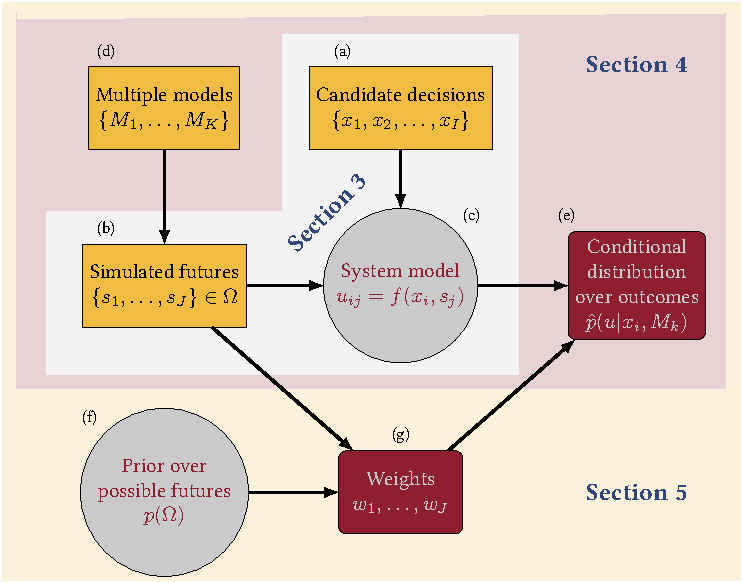
\includegraphics[width=\textwidth]{bayes-rdm.pdf}
  \caption{
    Outline of the proposed decision-analytic framework.
    In \cref{sec:analysis-explore} we use an exploratory framework to quantify the performance (c) of candidate decisions (a) under a large ensemble of possible futures (b).
    In \cref{sec:analysis-condition} we illustrate the ``multiple PDF problem'' by creating probability distributions over outcomes (e) that are conditional upon specific models describing the likelihood of different futures (d).
    In our case study, these are \gls{rcp} scenarios and physical models of sea level rise.
    Finally in \cref{sec:analysis-synthesize} we propose a subjective Bayesian framework for synthesizing across deep uncertainties by re-weighting sampled futures (f).
  }\label{fig:flowchart}
\end{figure}

\subsection{Explore}\label{sec:analysis-explore}

A first analytical step is to use the model in an ``exploratory'' mode.
Exploratory modeling is averse to making explicit assumptions about the likelihood of different \glspl{sow} and instead seeks to generate new knowledge \cite{bankes:1993} by systematically exploring a large number of possible futures, emphasizing interactions between different uncertainties \cite{reed_msdbook:2022}.
Exploratory modeling is often paired with analyses that identify relevant scenarios  \cite{lamontagne_discovery:2018,groves_scenarios:2007} or summarize a system's response to forcing \cite{Poff:2015jn,Steinschneider:2015kk,sriver_sealevel:2018}.
Despite the aversion to strong assumptions about the likelihood of different futures, subjective modeling decisions such as the choice of system model, the set of candidate decisions, the criteria used to assess outcomes, and the choice of how to sample \glspl{sow} can strongly influence results \cite{quinn_exploratory:2020}.

\subsection{Condition}\label{sec:analysis-condition}

Although exploratory modeling is a useful framework for understanding systems, there are many questions that it cannot answer.
For example, answering questions like ``what is the 95th percentile of metric $u$ under decision $x$'' or ``which decision minimizes expected damages'' or ``what is the probability of exceeding a critical threshold'' requires constructing estimators for the probability distribution over outcomes \cite<see>[for a general discussion]{schneider_scenarios:2002}.

One way to interpret an ensemble of \glspl{sow} is as \gls{iid} draws from some true data generating process.
This commonly arises when a single deep uncertainty (\eg, an emissions pathway) is used as an input for a fully probabilistic model; we call this scenario-conditional probabilistic analysis.
We add this concept to our framework with boxes (d) and (e) of \cref{fig:flowchart}, denoting the particular scenario (\ie, the assumed input) $M_k$.
If the \glspl{sow} are drawn \gls{iid} from $M_k$, the set of outcomes $u_{i, j}$ can be interpreted as \gls{iid} draws from the conditional distribution over outcomes, $p(u | x_i, M_k)$, allowing estimation of descriptive metrics.
This approach allows for quantification of uncertainty \emph{within} models of deeply uncertain processes, but can only qualitatively characterize uncertainty \emph{between} models \cite{wong_nola:2017,ruckert_coastal:2019,sharma_rcp:2021}.

We can also use this approach to understand \gls{dmdu} methods that sample a set of parameters from fixed ranges.
For example, \citeA{sriver_sealevel:2018} sample parameters describing the rate of \gls{slr} across a range of values to inform coastal adaptation.
Similarly, \citeA{trindade_waterpathways:2020} checks the performance of candidate decisions against an ensemble of synthetic time series of streamflow, water demand, and other parameters by sampling parameters that transform the available data over a plausible range \cite<\ie, robustness metrics; see>[for details]{mcphail_robustness:2019,herman:2015}.
Since sampling over a range is equivalent to sampling from a Uniform distribution, this assumption is equivalent to assuming the true inputs to come from independent Uniform distributions (one for each parameter) bounded by the plausible range.

Our primary concern is not that subjective assumptions about the likelihood of different futures are wrong -- this is, almost surely, inevitable -- but that when these assumptions are opaque and presented without critique or validation they may lead to inscrutable decision processes and sub-optimal decisions.

\subsection{Synthesize}\label{sec:analysis-synthesize}

As discussed in the previous subsection, estimating the expectation of arbitrary functions under uncertainty is a critical component of decision making under uncertainty.
If the \glspl{sow} are drawn \gls{iid} from the true distribution, then the expected value of some function  $f$, $\mathbb{E}\qty[f(\vb{s})]$, can be readily estimated as $\frac{1}{N} \sum_{j=1}^N f(\vb{s}_j)$.
However, this is often not the case; for example, a fixed set of simulations may be available for analysis or low-probability but high-impact regions of the parameter space may have been sampled.
In this case, the formula must be adjusted to
\begin{equation}
  \mathbb{E}\qty[f(\vb{s})] \approx \frac{1}{N} \sum_{i=j}^N w_j f(\vb{s}_j),
\end{equation}
where the $w_j$ are suitably chosen weights such that their sum is equal to 1.

The challenge then becomes to suitably estimate the $w_j$.
Paralleling joint probability methods for statistical analysis of tropical cyclones, we use a grid-based approach \cite{johnson_clara:2013,resio_probabilities:2007,toro_jpm-os:2010}.
First, we project the \glspl{sow} $\vb{s} \in \Omega$ onto a low-dimensional representation, which we denote $\qty{\psi_1, \psi_2, \ldots, \psi_J} \in \Psi$.
Then, we partition the parameter space into a region corresponding to each \gls{sow} and integrating the \gls{pdf} $p_\mathrm{belief}$ over each region.

We present here the case where the $\psi_j$ are one-dimensional; extensions to higher dimensions are possible.
We first sort the $\psi_j$  from least to greatest so that $\psi_{j-1} \leq \psi_j$, ($j \neq 1$).
Defining $F_\mathrm{belief}(s)$ to be the cumulative distribution corresponding to $p_\mathrm{belief}$, we calculate weights as
\begin{equation}\label{eq:weights}
  w_j = \begin{cases}
    F_\mathrm{belief}\qty(\frac{1}{2}\qty[\psi_1 + \psi_2])                                                                     & j = 1     \\
    F_\mathrm{belief}\qty(\frac{1}{2}\qty[\psi_{j} + \psi_{j+1}]) - F_\mathrm{belief}\qty(\frac{1}{2}\qty[\psi_{j-1} + \psi_j]) & 1 < j < J \\
    1 - F_\mathrm{belief}\qty(\frac{1}{2}\qty[\psi_{J-1} + \psi_J])                                                             & j = J.
  \end{cases}
\end{equation}
This step is illustrated in \cref{fig:grid-sketch}.
Diagnostic checks, such as examining the histogram of weights (not shown), may be valuable protections against degeneracy.

\begin{figure}
  \centering
  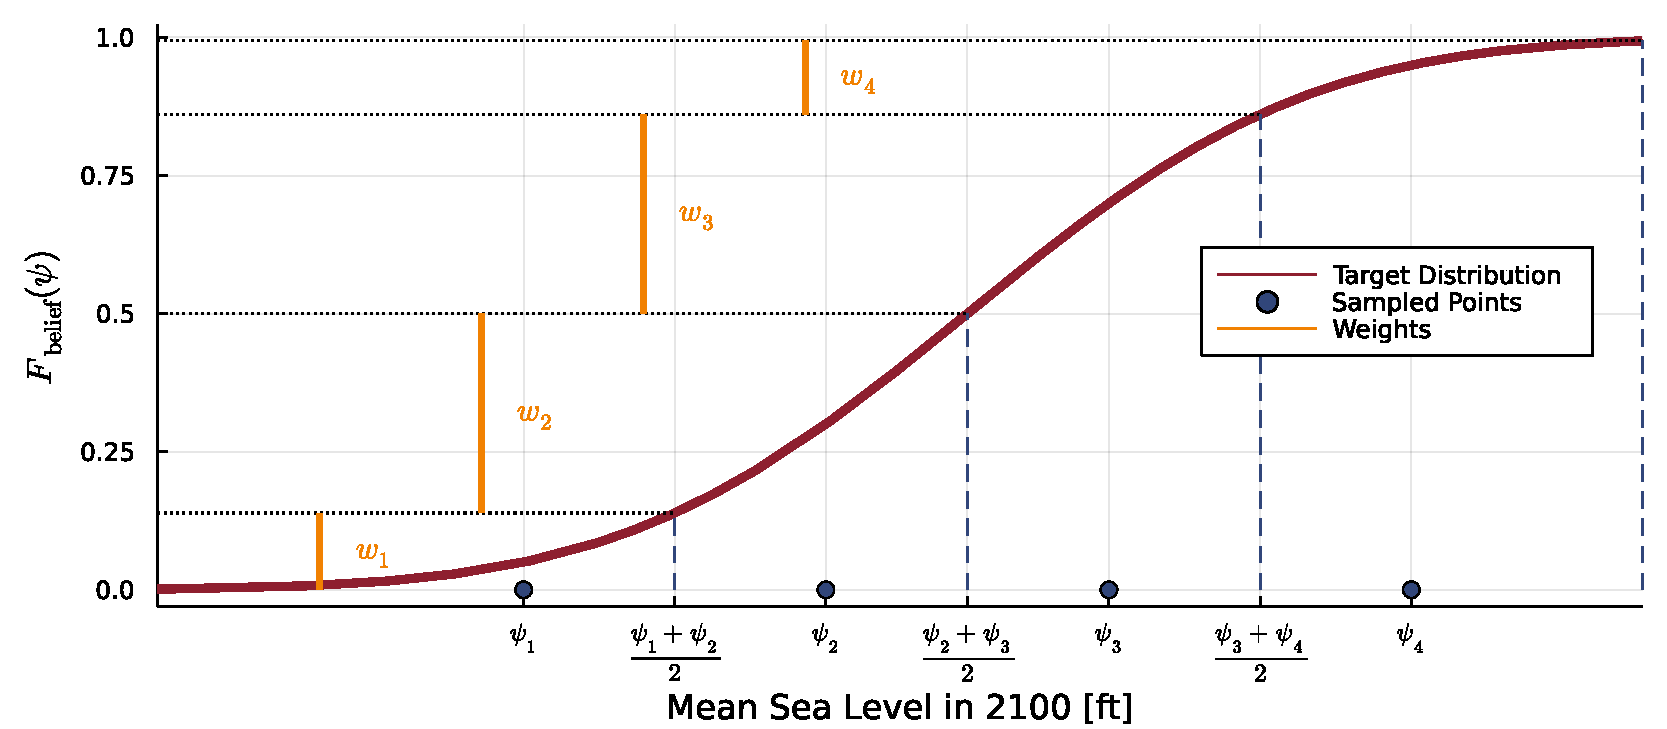
\includegraphics[width=\textwidth]{grid-sketch}
  \caption{
    Schematic of \gls{sow} weighting scheme defined in \cref{eq:weights}.
    This method is illustrated for a hypothetical target distribution (dark red line) and $J=4$ samples $\psi_1, \psi_2, \psi_3, \psi_4$ (blue dots).
    As shown in \cref{eq:weights}, the weights $w_j$ (orange vertical lines) are calculated based on the cumulative distribution function of the target distribution at the halfway points $\frac{1}{2}\qty[\psi_j+\psi_{j+1}]$ (vertical dashed lines).
  }\label{fig:grid-sketch}
\end{figure}

The aim of this re-weighting framework is to integrate an ensemble of \glspl{sow} used for exploratory modeling into formal decision analysis, even when the \glspl{sow} deliberately over- or under-sample some regions of the parameter space.
As in \cref{sec:analysis-condition}, we must condition on a model: where the analysis of \cref{sec:analysis-condition} conditions upon deep uncertainties, the approach outlined in this subsection synthesizes across them.
We reiterate that stakeholders and experts will not, in general, agree on $p_\mathrm{belief}$ because there is not, even conceptually, an objectively correct choice \cite{oreskes_verification:1994,walker_deep:2013}.
However, we posit that since we cannot be ``right,'' it is valuable to maximize the transparency of our implicit probabilistic assumptions, and suggest that writing down an explicit model for $p_\mathrm{belief}$ supports this aim.

\section{Demonstrating the concept with a case study}\label{sec:case-study}

To illustrate the proposed decision analytic framework, we model a one-time decision of whether to elevate a house, and if so by how much (\cref{fig:xlrm}).
Following the approach outlined in \citeA{zarekarizi_suboptimal:2020}, we focus on a case study of a \emph{hypothetical} house in Norfolk, VA.
For interpretability, we focus on deep uncertainty in \gls{msl} and approximate other model parameters as shallow uncertainties as shown in \cref{tab:uncertainties}.
We use the notation developed in the previous section to describe the case study.
Specifically,
\begin{enumerate}
  \item The decision vector $\vb{x}$ is comprised of discrete possible house heightenings ($\Delta h$); we consider $\Delta h = \qty{\SI{0}{ft}, \SI{0.25}{ft}, \ldots, \SI{12}{ft}}$.
  \item The \glspl{sow} describe annual time series of \gls{msl} over the $T=70$ year house lifetime so $\vb{s} \in \mathbb{R}^T$
  \item The system model $f$ quantifies up-front costs (the cost of elevating) and lifetime expected damages (the structural cost of experiencing floods), given a decision $x_i$ and \gls{sow} $s_j$, by integrating economic and engineering damage models over a probability distribution for storm surge. We elaborate upon these metrics in \cref{sec:case-metrics}.
\end{enumerate}
In the remainder of this section we describe data sources and treatment of \gls{slr} (\cref{sec:case-slr}), storm surge (\cref{sec:case-surge}), damages and metrics (\cref{sec:case-metrics}), and finally the subjective priors $p_\mathrm{belief}$ used to apply the re-weighting method described in \cref{sec:analysis-synthesize} to this case study (\cref{sec:case-priors}).

\begin{table}
  \centering
  \caption{
    Summary of parameters, their notation, and how their uncertainty is represented.
    Symbols describing the decision-analytic framework are described in \cref{fig:flowchart}.
  }\label{tab:uncertainties}
  \footnotesize
  \begin{tabular}{p{1.25in} p{0.75in} p{3in}}
    \toprule
    Name                 & Symbol            & Uncertainty                                                                          \\
    \midrule
    \Gls{msl}            & $\overline{y}(t)$ & Deeply uncertain: four physical models $\times$ four \acrshort{rcp} scenarios        \\
    Storm surge          & $y'(t)$           & Probabilistic: Bayesian inference on a stationary \acrshort{gev} model               \\
    Annual maximum flood & $y(t)$            & Deterministic: $y(t)=\overline{y}(t)+y'(t)$                                          \\
    Discount rate        & $\rho$            & Determinitic: 2.5\% per year                                                         \\
    Depth-damage         & $D(h-y)$          & Deterministic: based on HAZUS model \cite<see>[]{zarekarizi_suboptimal:2020}         \\
    Elevation cost       & $C(\Delta h)$     & Deterministic: a piecewise linear model following \citeA{zarekarizi_suboptimal:2020} \\
    Initial height       & $h_0$             & Deterministic: \SI{1}{ft} below the \gls{bfe}, unless otherwise noted                \\
    House floor area     & --                & Deterministic: \SI{1500}{ft^2}                                                       \\
    Structural value     & --                & Deterministic: \usd{200000}                                                          \\
    House lifespan       & $T$               & Deterministic: 70 years                                                              \\
    \bottomrule
  \end{tabular}
\end{table}

\begin{figure}
  \centering
  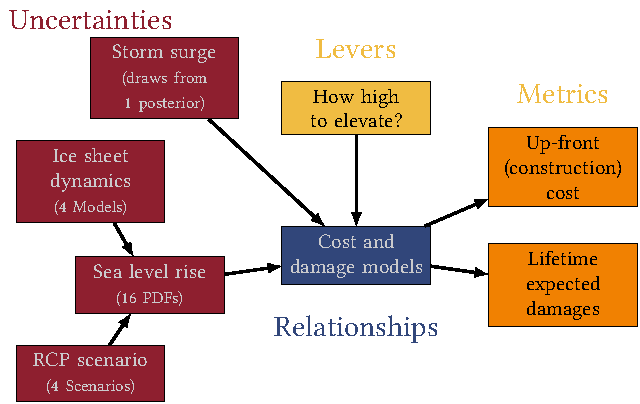
\includegraphics[width=\textwidth]{xlrm.pdf}
  \caption{
    Conceptual diagram of the considered example.
    A \acrfull{sow} consists of a description of the uncertain factors (red).
    We model a problem with a single lever (yellow), which is how high to elevate a house ($\Delta h$).
    For each \acrshort{sow} (red) and each value of $\Delta h$, the system model (blue) is used to calculate performance metrics (gray).
    We also compute a third metric, expected lifetime costs, which is the sum of up-front costs and lifetime expected damages.
  }\label{fig:xlrm}
\end{figure}

\subsection{\Glsentrylong{slr}}\label{sec:case-slr}

We analyze simulations of \gls{msl} at Sewells Point, VA from four probabilistic physical models using data published in \citeA{ruckert_coastal:2019}.
The four models considered are (i) the BRICK model (version 0.2) with slow (``BRICK Slow'') and (ii) fast (``BRICK Fast'') ice sheet dynamics \cite{wong_brick0.2:2017}, (iii) the \citeA{kopp_probabilistic:2014} model (``K14''), and (iv) the \citeA{deconto_antarctica:2016} model (``DP16'').
The \citeA{kopp_probabilistic:2014} and \citeA{deconto_antarctica:2016} models have a ten year time step, which we linearly interpolate onto a one year time step for consistency.
These four models represent physical processes, particularly of ice sheet dynamics, in different ways.
The differences in these models leading to diverging estimates of how \gls{msl} responds to temperature.
For a discussion of these model outputs we refer the reader to \citeA{ruckert_coastal:2019}.

Estimates of nonstationary \gls{msl} also depend on anthropogenic forcing, which is itself deeply uncertain \cite{ho_scenarios:2019,srikrishnan_probabilistic:2022}.
To sample this uncertainty, we use simulations from each physical model under four \gls{rcp} scenarios, yielding sixteen time-varying distributions of \gls{msl}.

\begin{figure}
  \centering
  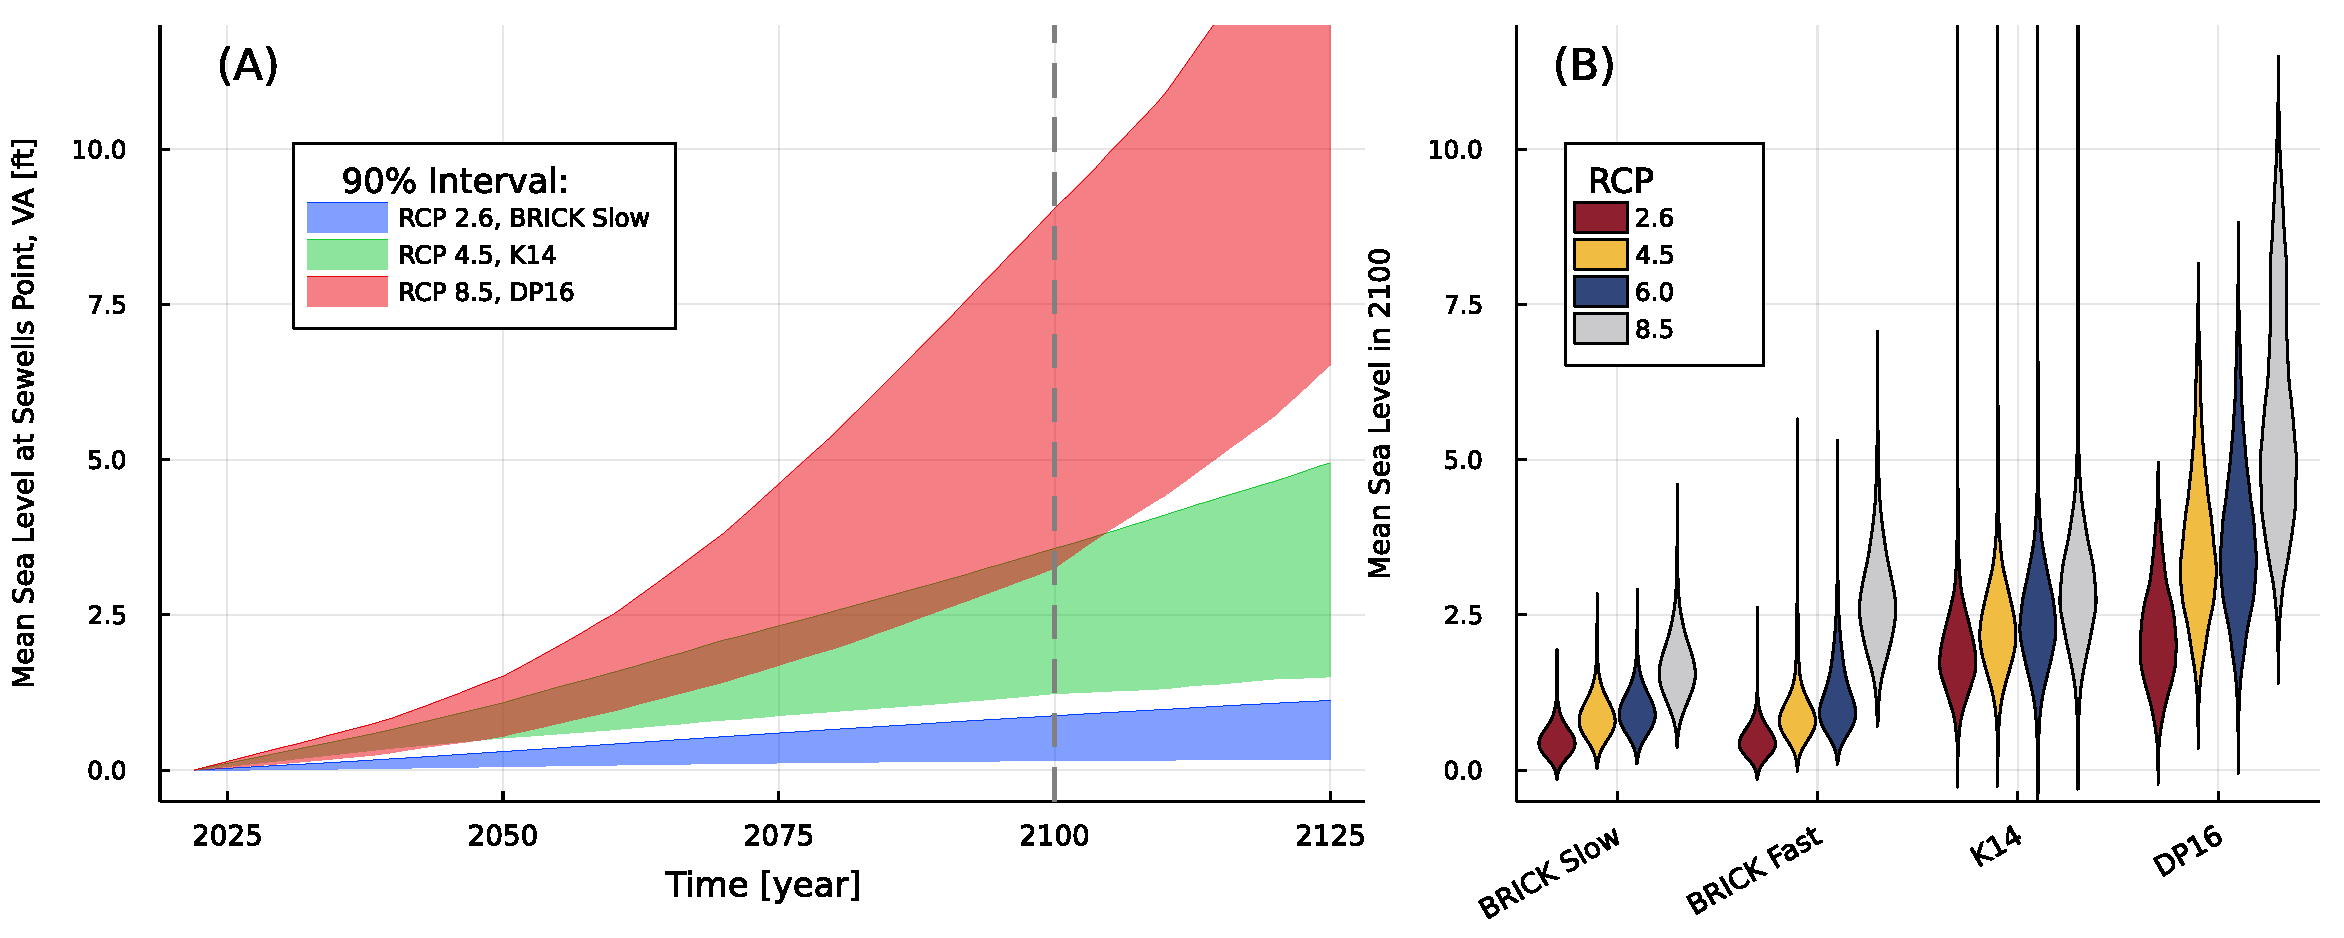
\includegraphics[width=\textwidth]{lsl-evolution}
  \caption{
    Projections of future mean sea level depend strongly on the choices of physical model and forcing.
    (A): 90\% confidence intervals for mean sea level at Sewells Point, VA as a function of time for a representative subset of three probabilistic models (out of sixteen).
    (B): probability distribution of \gls{msl} at Sewells Point, VA in the year 2100 for each probabilistic model considered.
  }\label{fig:lsl-evolution}
\end{figure}

The choices of physical model and \gls{rcp} scenario jointly determine future \gls{msl} $p(\overline{y}|t)$.
\Cref{fig:lsl-evolution}(a) shows the time-varying 90\% credible intervals of \gls{msl} for three representative models.
The divergence between the the best-case (blue) and worst-case (red) models is small in the early 21st century and increases rapidly thereafter.
\Cref{fig:lsl-evolution}(b) shows the \glspl{pdf} of mean sea level in 2100 (dashed vertical line in panel (a)) under each of the sixteen models considered.
We return in \cref{sec:results-conditional} to the challenge of decision making under multiple \glspl{pdf}.

\subsection{Storm surges}\label{sec:case-surge}

Following prior work \cite<\eg,>[]{garner_slrise:2018,sriver_sealevel:2018}, we model annual maximum floods $y(t)$ as the sum of sea level $\overline{y}(t)$, described in the previous subsection, and annual maximum storm surges $y'(t)$, neglecting hydrodynamic effects.

We use data on storm surge at Sewells Point, VA (gauge 8638610) from the \gls{noaa} tides and currents data archive \cite{noaa_tidesandcurrents:2022}.
Hourly recordings of water level are available from 1928 to the present; we use data from the period January 1, 1928 to December 31, 2021.
For each calendar year we first remove the annual mean, then calculate the maximum water level.
We refer this time series of annual maximum storm surges as $y'(t)$.
We display this time series of annual maxima storm surges in \cref{fig:surge-obs-return}(a).
The largest recorded surge was the Chesapeake-Potomac hurricane of 1933, which caused a surge of over \SI{7}{ft} at this gauge, but other hurricanes and Nor'easters have caused surges above \SI{6}{ft}.

\begin{figure}
  \centering
  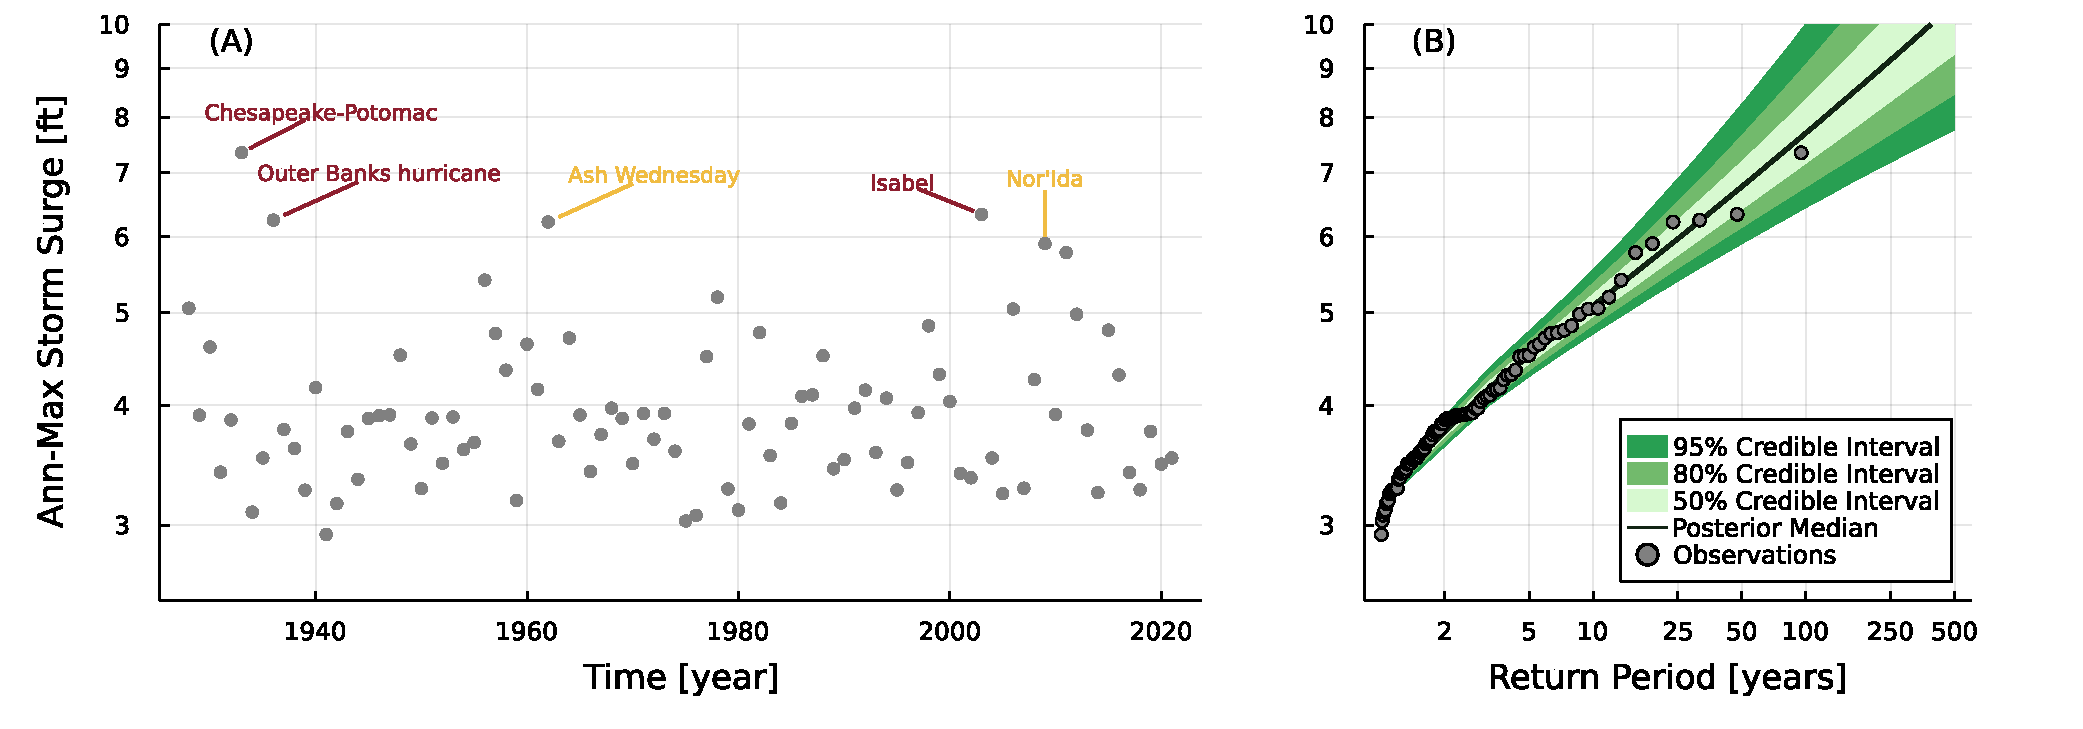
\includegraphics[width=\textwidth]{surge-obs-return}
  \caption{
    Annual maximum storm surges (after subtracting \acrlong{msl}) at Sewells Point, VA from the freely available NOAA tides and currents data archive \protect\cite{noaa_tidesandcurrents:2022}.
    (A):
    time series of historic storms.
    Red (yellow) arrows denote notable tropical cyclones (Nor'easters).
    (B):
    return periods.
    Dots indicate observed values; their $x$-value is their plotting position using the Weibull formula (eq.~\ref{eq:weibull}).
    Gray lines show the 50, 80, and 95\% posterior confidence intervals from the Bayesian \gls{gev} fit (\cref{sec:case-surge}).
  }\label{fig:surge-obs-return}
\end{figure}

We model future storm surge using a stationary \gls{gev} model:
\begin{equation}\label{eq:surge-model}
  y'(t) \sim \text{GEV}\qty(\mu, \sigma, \xi),
\end{equation}
where $y'(t)$ is the storm surge (above \gls{msl}) in year $t$ and a \gls{gev} distribution with location, shape, and scale parameters $\mu$, $\sigma$, and $\xi$, respectively, has the probability density function given in \cref{eq:gev-dist}.
This model assumes stationarity, neglecting any potential time dependence.

Our approach to model assessment is based on the concept of principled workflow design for model building and checking \cite<see>[for details]{gelman_workflow:2020}.
One model choice, analogous to the choice of statistical distribution or the assumption of stationarity, is the choice of how to represent prior information.
We include two forms of prior information.
First, we constrain the shape parameter to be positive, $\xi > 0$, to reflect knowledge about the support of $y'$, which for a variable distributed according to \cref{eq:gev-dist} is:
\begin{equation*}
  \mathrm{supp}~ y' =
  \begin{cases}
    \xi < 0: & y' \in \qty(-\infty,~ \mu - \nicefrac{\sigma}{\xi}) \\
    \xi > 0: & y' \in \qty(\mu-\nicefrac{\sigma}{\xi},~ \infty).
  \end{cases}
\end{equation*}
Since storm surges cannot be negative, only the latter is physically defensible, justifying our choice to constrain the shape parameter to be positive.
Second, we add weakly informative priors.
Rather than applying prior information directly over the joint distribution of the parameters $\qty{\mu,\sigma,\xi}$, we instead apply a prior over extreme quantiles of the distribution, as in \citeA{coles_evd:1996}.
Specifically, we apply Inverse Gamma priors over the 2, 10, 100, and 500 year return levels, with means of \SIlist{4;6;10;15}{ft} and standard deviations of \SIlist{1.5;1.75;2.25;2.75}{ft}, respectively.
The parameters of the Inverse Gamma distribution can be calculated from these moments (see eq.~\ref{eq:inv-gamma-params}).
These means and standard deviations were chosen to represent plausible physical ranges (\cref{fig:surge-gev-priors}).

For inference, we draw \num{10000} samples from the posterior distribution $p(\mu,\sigma,\xi | y')$ using Hamiltonian Markov Chain Monte Carlo \cite{betancourt_hamiltonian:2018,hoffman_nuts:2011} implemented in the Turing package of the Julia programming language \cite{perkel_julia:2019,ge_turing:2018,tarek_dynamicppl:2020,besancon_distributions.jl:2021,bezanson_julia:2012}.
Diagnostics suggest (though cannot guarantee) convergence (see \cref{tab:surge-posterior-mcmc-diagnostics}).
We evaluate the model's fit using posterior predictive checks \cite<see>[section 2.4 and references therein]{gelman_workflow:2020}.
Using the lag 1 and 2 partial autocorrelations, sample maximum, sample minimum, sample median, and Mann-Kendall test value as Bayesian test statistics, we find that draws from the posterior predictive distribution match the observed test statistics credibly (\cref{fig:surge-test-statistics}) although panels (a) and (b) suggest the possibility of temporal structure not captured by our stationary \gls{iid} model.
Future efforts could represent this structure by conditioning the parameters of the distribution on relevant climate indices \cite<as in>[]{wong_surge:2018,farnham_orbrep:2018,farnham_jetstream:2017,ossandon_semibayesian:2021}.

Other model validations lend confidence to the stationary \gls{gev} model selected.
For example, \cref{fig:surge-obs-return}(b) shows the estimated return periods for these storm surges; the estimated return period  (shading) matches the the empirical plotting position (dots) and a positive control test (\cref{fig:surge-synthetic-data-experiment}) validates the model's ability to recover known parameter values.

\subsection{Damages and metrics}\label{sec:case-metrics}

The system model (``relationships'' in \cref{fig:xlrm}) is comprised of two key pieces.
The first is a fragility model that estimates the expected flood damages for a particular year (``expected annual damages''), given the elevation of the house and the mean sea level for that year.
The second model converts a time series of annual expected damages into lifetime expected damages.

We define expected annual damages in year $t$ as the expectation of the damage function with respect to storm surge.
This expectation depends on the house's height ($h = h_0 + \Delta h$) where $h_0$ is the initial height relative to the gauge and $\Delta h$ is the amount by which the house is elevated.
The expected annual damage is thus
\begin{equation}\label{eq:ead}
  \textrm{EAD}(t) = \mathbb{E}[D \qty(h-\overline{y}(t))] = \int_{y'} p(y') D \qty(h - \qty(\overline{y}(t) + y')) \dd{y'},
\end{equation}
where $D(h-y)$ is a deterministic function specifying damage as a function of flood depth (relative to the house).
Following \citeA{zarekarizi_suboptimal:2020}, we use the \gls{hazus} depth-damage curves provided by \gls{fema}; this depth-damage relationship is shown in \cref{fig:cost-depth-damage}.
For comparison, \cref{fig:cost-depth-damage} also shows the ``Europa'' depth-damage relationship developed by the Joint Research Center of the European Commission's science and knowledge service \cite{huizinga_depthdamage:2016}.
Although \citeA{zarekarizi_suboptimal:2020} demonstrate that the choice of fragility function is important for informing house elevation, we use only the HAZUS model for simplicity.

The expected annual damage is sometimes calculated by assuming analytically tractable functional forms for the depth-damage relationship and for the  distribution of hazard \cite<\eg,>[]{vandantzig_dike:1956}.
However, the convolution of the HAZUS depth-damage equation with the \gls{gev} posterior does not have a tractable analytic solution.
Instead, we estimate this convolution through a Monte Carlo method (see \cref{sec:alg-ead} for details).
Then, because the expectation in \cref{eq:ead} depends only on $h-\overline{y}(t)$, we calculate expected annual damages for a wide range of possible heights, then use this to train a computationally efficient surrogate model (using linear interpolation; see \cref{sec:surrogate-ead}).

The second component of the system model converts a time series of $\mathrm{EAD}$ into lifetime expected damages, which we define as the up-front  discounted sum of expected annual damages:
\begin{equation}\label{eq:led}
  \textrm{LED} = \sum_{t=t_i}^{t_f} \gamma^{\qty(t-t_i)} \textrm{EAD}(t),
\end{equation}
where  $\gamma = 1- \rho$ ($\rho$ being the discount rate), the initial time $t_i=2022$, and the end time $t_f = t_i + T - 1$.
Although \citeA{zarekarizi_suboptimal:2020} show that uncertainty in the discount rate is important for decision support, we use a fixed discount rate (see \cref{tab:uncertainties}) for the purposes of this didactic study.
For a more theoretical discussion see \citeA{arrow_discount:2013}.

To assess the performance of a given decision for a specific \gls{sow} (``Metrics'' in \cref{fig:xlrm}), we calculate the following metrics for each decision-\gls{sow} combination:
\begin{enumerate}
  \item ``Up-front cost'' is the cost of elevating a house. Following \citeA{zarekarizi_suboptimal:2020}, we use estimates of construction cost from the Coastal Louisiana Risk Assessment \cite{fischbach_clara:2012}. We normalize this cost by house value; this cost curve is shown in \cref{fig:cost-up-front}.
  \item ``Lifetime expected damages'' is calculated following \cref{eq:led}.
  \item ``Expected lifetime costs'' is the sum of lifetime expected damages and up-front costs.
\end{enumerate}

\subsection{Prior over \glsentrylong{slr}}\label{sec:case-priors}

We construct three probabilistic models for $p_\mathrm{belief}(\psi)$, which represents the amount of \gls{slr} from 2022 to 2100.

We use a Gamma distribution for all three priors, parameterized following \cref{eq:gamma-dist}.
\Cref{tab:slr-priors} specifies the parameters of these distributions, as well as some quantiles of the distributions.
Their \glspl{pdf} are also plotted in \cref{fig:lsl-priors-weights}(A).

\begin{table}[ht]
  \centering
  \caption{
    Subjective priors over \gls{slr} from 2022 to 2100, \ie $p_\mathrm{belief}(\psi)$.
    The name of the distribution, the parameters of the Gamma distribution with shape $\alpha$ and scale $\theta$, and the 2.5, 25, 50, 75, and 97.5th percentiles (values in \si{ft}).
  }\label{tab:slr-priors}
  \begin{tabular}{llllllll}
    \toprule
    Name          & \multicolumn{2}{c}{Parameters} & \multicolumn{5}{c}{Percentiles (in \si{ft})}                                     \\
    \cmidrule(lr){2-3}
    \cmidrule(lr){4-8}
                  & $\alpha$                       & $\theta$                                     & 2.5  & 25.0 & 50.0 & 75.0 & 97.5  \\
    \midrule
    Slow SLR      & 1.75                           & 0.50                                         & 0.08 & 0.39 & 0.72 & 1.19 & 2.57  \\
    Uncertain SLR & 1.75                           & 1.25                                         & 0.21 & 0.98 & 1.79 & 2.97 & 6.41  \\
    Rapid SLR     & 3.50                           & 1.25                                         & 1.06 & 2.66 & 3.97 & 5.65 & 10.01 \\
    \bottomrule
  \end{tabular}

\end{table}

We developed these priors for didactic purposes, to illustrate a range of possible beliefs.
We can compare them, for example, with analysis published by \gls{noaa}, which project \SIlist{1.94;2.62;4.27;5.25;6.89}{ft} for the low, intermediate, low intermediate, intermediate high, and high scenarios, respectively \cite[table.~2.4]{sweet_slr:2022}.
We can also compare to the analyses of \citeA{sriver_sealevel:2018} which uses a rescaled Beta distribution with bounds of \SIrange{0.83}{8.2}{ft} and a most plausible estimate of \SI{3.1}{ft}.
Our samples bound all of these estimates.

\section{Results and discussion}\label{sec:results}

We illustrate our approach to synthesizing uncertainties by sequentially analyzing the house elevation problem through the lenses of exploratory modeling (\cref{sec:results-exploratory}), scenario-conditional analysis (\cref{sec:results-conditional}), and finally the proposed synthesis method (\cref{sec:results-synthesis}).

\subsection{Exploratory modeling}\label{sec:results-exploratory}

We begin by using our model in an ``exploratory'' mode with an aim of learning about interactions between system dynamics and decisions.

\begin{figure}
  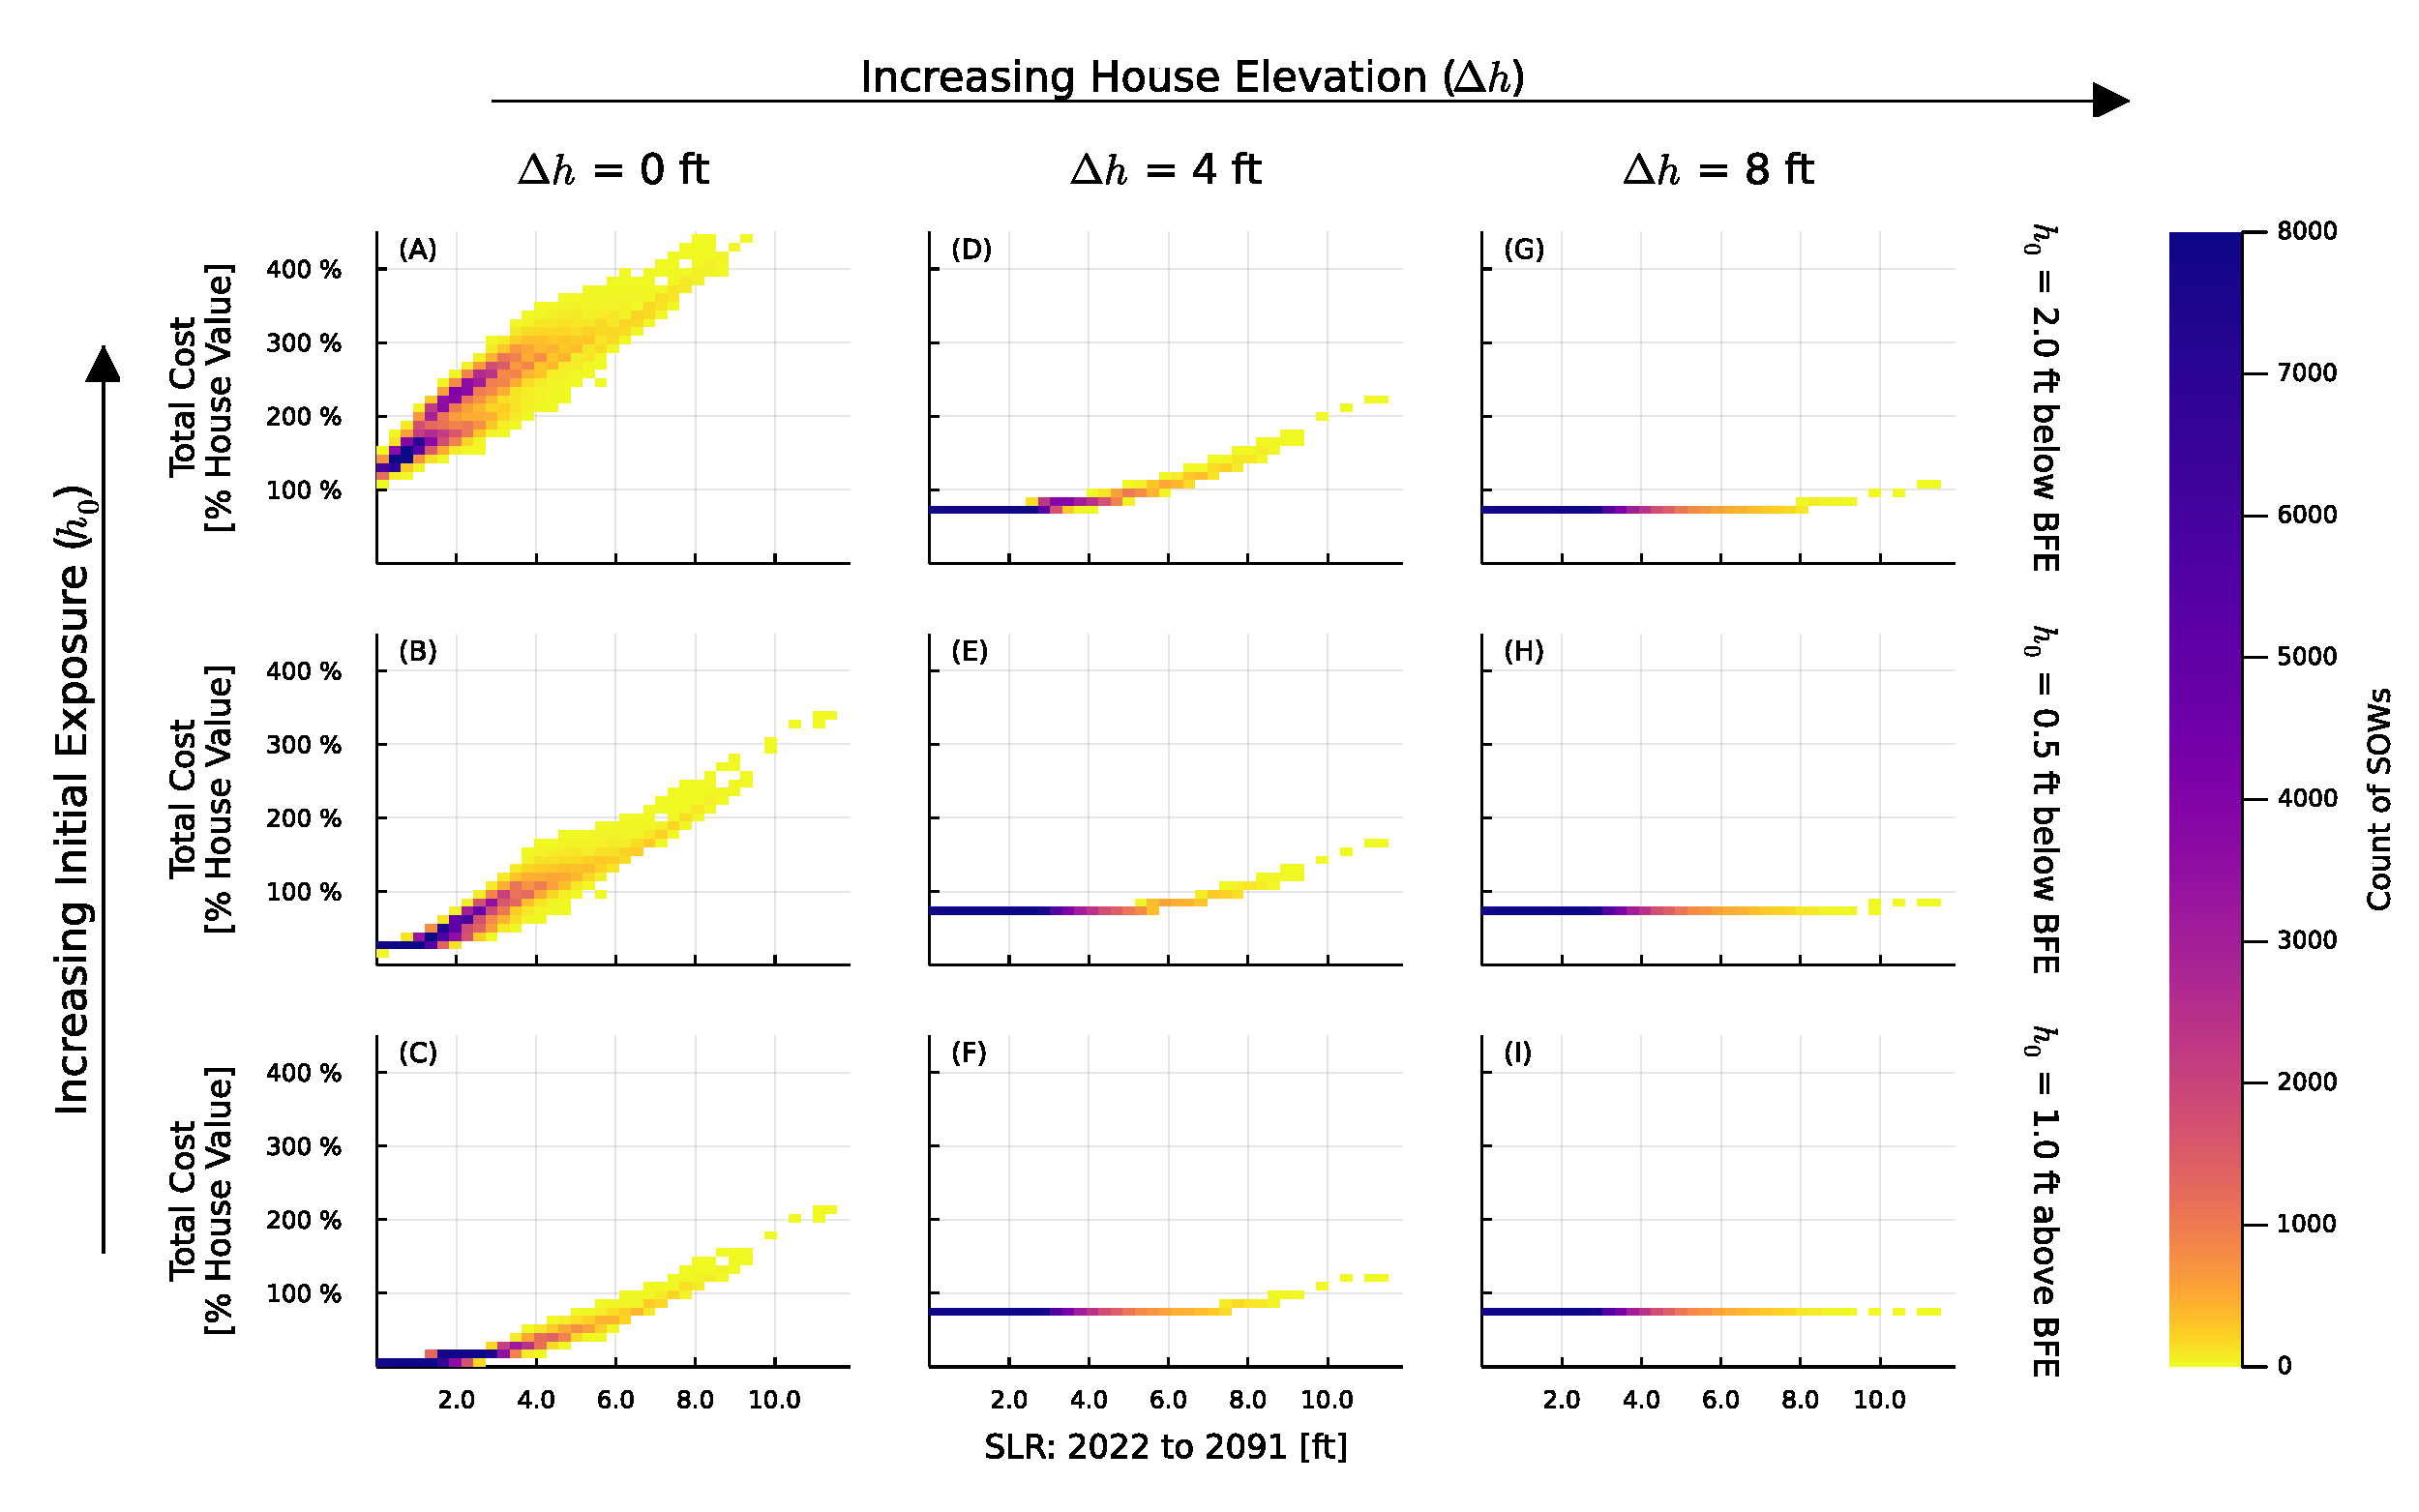
\includegraphics[width=\textwidth]{scenario-map-slr-cost}
  \caption{
    Scenario maps show the dependence of expected lifetime cost (damages plus up-front cost) as a function of \acrfull{msl} in 2100 for several values of initial height ($h_0$) and house elevation ($\Delta h$).
    Colors indicate the number of \acrfullpl{sow} of falling within each box.
    The lowest-cost outcomes occur when exposure is low ($h_0$ is large and \acrfull{slr} is minimal) and the house is not elevated (no up-front cost).
    The highest-cost outcomes arise when exposure is high ($h_0$ is small and \gls{slr} is rapid) and investment is inadequate.
    In all cases, elevating the house reduces the variance in total lifetime cost.
    Values are sensitive to model constants; see \cref{tab:uncertainties}.
  }\label{fig:scenario-map-slr-cost}
\end{figure}

One application of exploratory analysis is to reveal the range and variation in outcomes, conditional on taking a particular decision.
\Cref{fig:scenario-map-slr-cost} shows the dependence of expected lifetime costs (damages plus up-front costs; $y$-axis) as a function of  \gls{slr} over the house lifetime ($x$-axis), height increase ($\Delta h$; columns), and initial elevation ($h_0$; rows).
The outcomes with lowest total lifetime costs arise when the house is not elevated ($\Delta h = 0$) and \gls{slr} is minimal (bottom left corners).
The outcomes with highest total lifetime costs arise when the house is elevated only slightly and \gls{slr} is rapid.
As $\Delta h$ increases, the best-case scenario becomes more expensive because up-front costs increase, but worst-case scenarios become less expensive because even if \gls{slr} is substantial, damages will be negligible.

This analysis answers ``what-if'' questions like ``given $h_0$ and $\Delta h$, what is the range of total costs a homeowner could face if \gls{slr} over the house lifetime is \SI{1}{ft} or \SI{10}{ft}.''
For some decision-makers, contextualizing this information against a few scenarios of \gls{slr} \cite<\eg, those of>[]{sweet_slr:2022} may prove sufficient for decision making.
However, this analysis does not shed light on cost-benefit analyses or return periods, nor does it permit quantitative comparison against other possible decisions unless strong implicit assumptions are made.

\subsection{Scenario-conditional optimization}\label{sec:results-conditional}

We now turn to the scenario-conditional analysis described in \cref{sec:analysis-condition}.
Whereas the exploratory analysis of the previous subsection interpreted each time series of future sea level as a sample from the space of possible futures, we can also interpret each \gls{sow} as a draw from one of the sixteen models of \gls{slr} shown in \cref{fig:lsl-evolution}.
As discussed in \cref{sec:analysis-condition}, this allows a formal estimation of decision metrics, conditional on the chosen scenario.

\begin{figure}
  \centering
  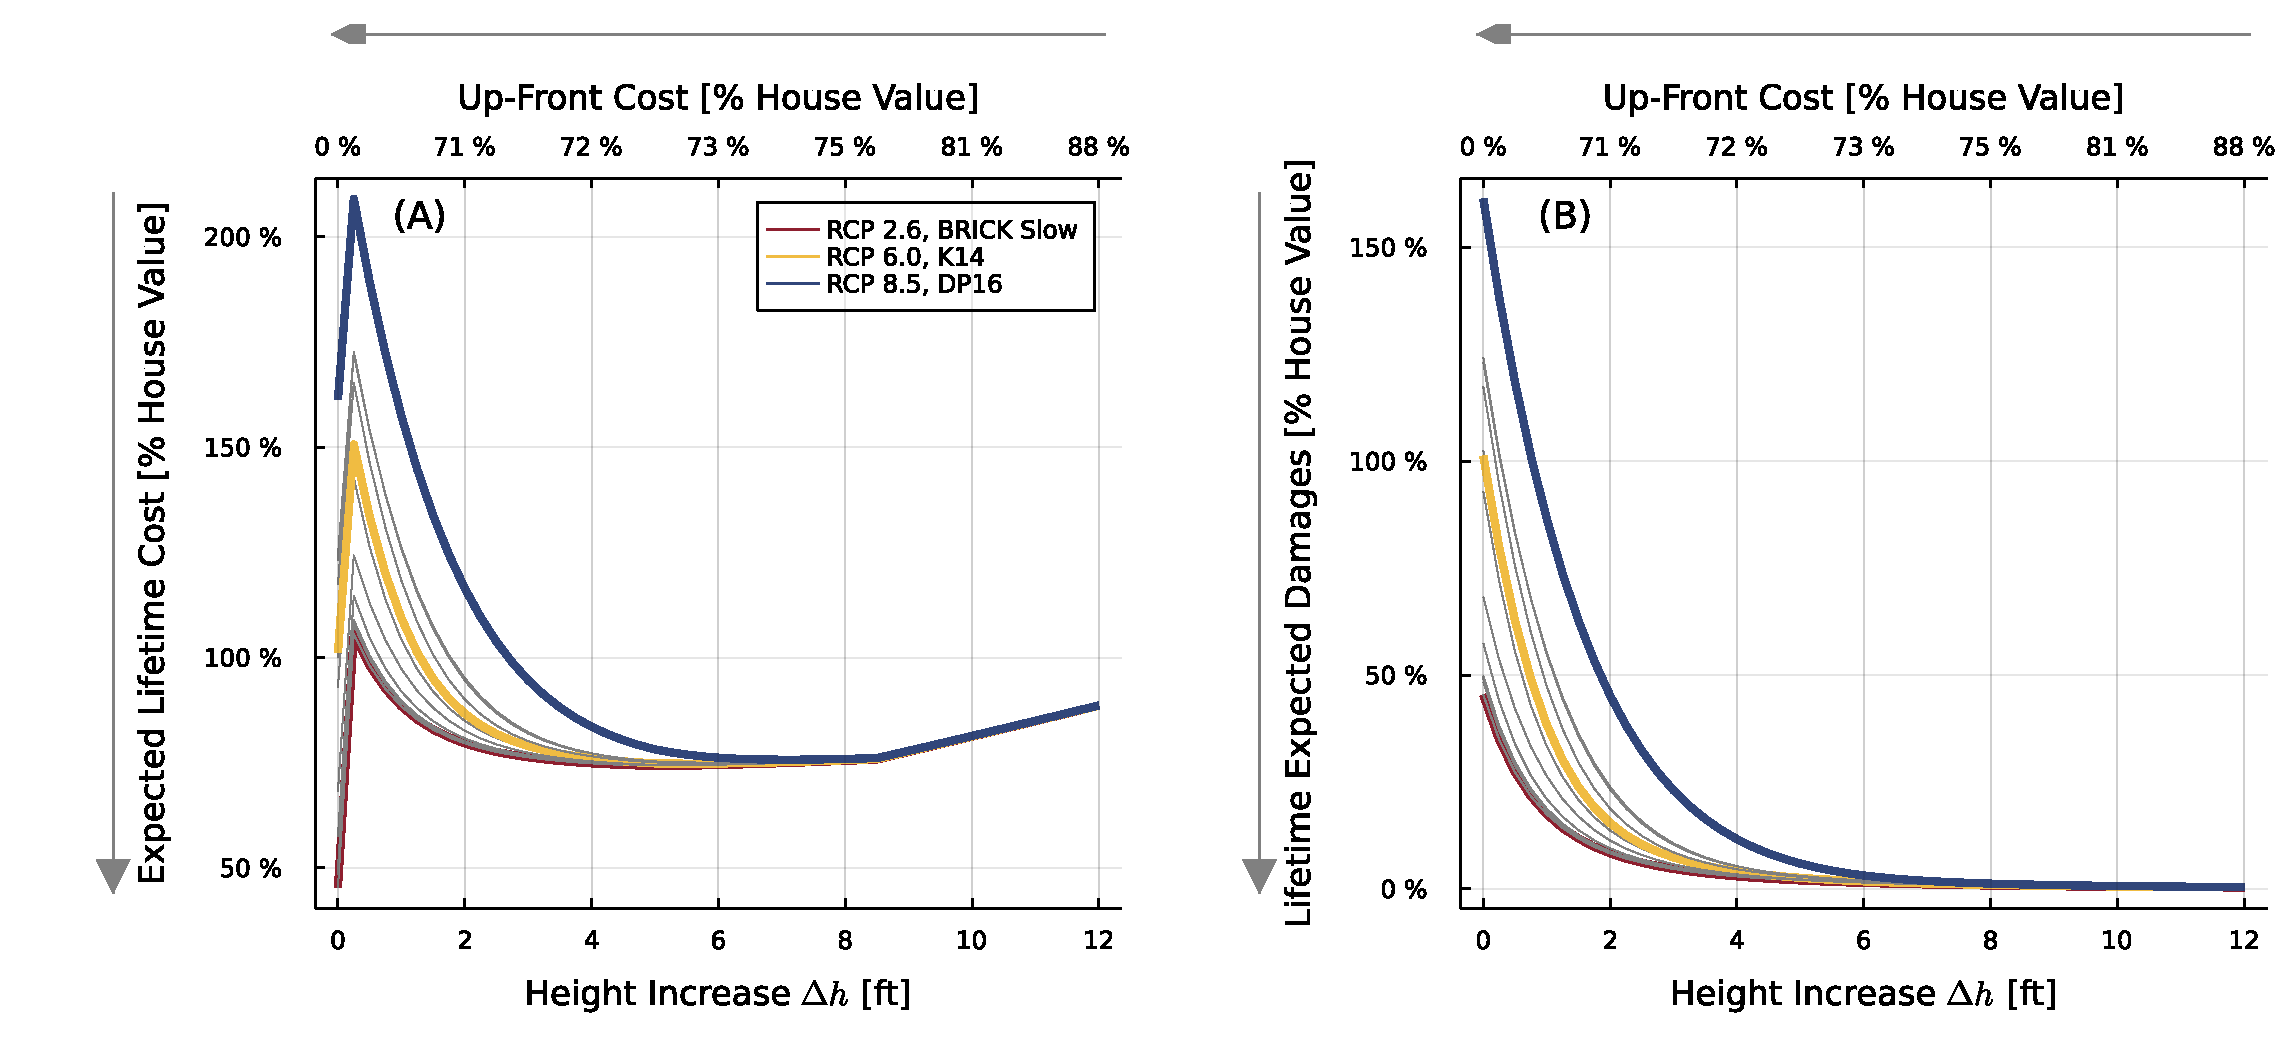
\includegraphics[width=\textwidth]{tradeoffs-by-rcp}
  \caption{
    Each probabilistic model or scenario leads to a different estimate of the Pareto frontier.
    For emphasis, we highlight three representative models: the Brick Slow model \protect\cite{wong_brick0.2:2017} under \gls{rcp} 2.6, the K14 \protect\cite{kopp_probabilistic:2014} model under \gls{rcp} 6.0 and the DP16 model \protect\cite{deconto_antarctica:2016,kopp_evolving:2017} under \gls{rcp} 8.5.
    (A): trade-off between up-front cost (which is a monotonic function of height increase) and expected lifetime costs.
    (B): trade-off between up-front cost and lifetime expected damages (eq.~\ref{eq:led}).
    Light gray lines show estimates for all 16 models (four \gls{rcp} scenarios times four physical parameterizations) considered.
    Colored lines highlight three representative models for emphasis.
    The gray arrows indicate the direction of preference.
  }\label{fig:tradeoffs-by-rcp}
\end{figure}

This probabilistic interpretation allows us to compute, for example, expected values.
For example, \cref{fig:tradeoffs-by-rcp}(a) plots the expected total lifetime cost as a function of $\Delta h$ for the sixteen models considered (we highlight three representative models).
Similarly, \cref{fig:tradeoffs-by-rcp}(b) plots the lifetime expected damages as a function of $\Delta h$.
For small $\Delta h$, expected costs are low under optimistic models (\eg, \gls{rcp} 2.6 with slow ice sheet dynamics; red lines) and high under pessimistic models (\eg, \gls{rcp}8.5 with the DP16 model; blue lines).
For example, under the most pessimistic model (blue line), the cost-minimizing height increase is \SI{6}{ft}, which incurs an up-front cost of 73\% of the house value but reduces lifetime expected damages by over 150\% of house value.
Under the most optimistic model (gray line), the cost-minimizing decision is to not elevate, as elevating \SI{6}{ft} incurs the same up-front cost yet reduces lifetime expected damages by less than 50\% of house value.

This approach is, in a sense, another form of exploratory modeling: instead of considering a very large ensemble of \glspl{sow}, we consider a much smaller set of probabilistic models.
This approach is attractive because it allows modelers to focus on their domain expertise (\eg, the response of ice sheets and global sea levels to a particular climate future).
However, conditioning simulations on a set of climate futures and physical models presents what we term ``the multiple \gls{pdf} problem'' because it leaves decision makers with many \glspl{pdf} to choose from and hence many trade-off curves to navigate.
The multiple \gls{pdf} problem has also been shown in other contexts.
For example, \citeA{sharma_rcp:2021} model the reliability of stormwater infrastructure under different climate models and downscaling methods, finding diverging estimates of future rainfall hazard, even under a single \gls{rcp} scenario.
Similarly, \citeA{wong_nola:2017} construct 18 probability distribution functions for future flood risk in New Orleans, considering multiple models for ice sheet dynamics and storm surge and multiple \gls{rcp} scenarios. As a last example, \citeA{haasnoot_sealevelrise:2021} identify global adaptation needs for different \gls{slr} scenarios.
Although this scenario-conditional analysis is appropriate for understanding differences between models, its key limitation is that it \textbf{places the burden for deciding which model to design for onto the end user.}

\subsection{Synthesizing deep uncertainties for decision analysis}\label{sec:results-synthesis}

The proposed approach can help overcome the limitations of scenario-conditional analysis.
We illustrate how the re-weighting method described in \cref{sec:analysis-synthesize} can help to shed light on climate risk management under deep uncertainty.
We present results using each of the models for $p_\mathrm{belief}$ outlined in \cref{sec:case-priors}.
These three distributions are shown in \cref{fig:lsl-priors-weights}(A).

\begin{figure}
  \centering
  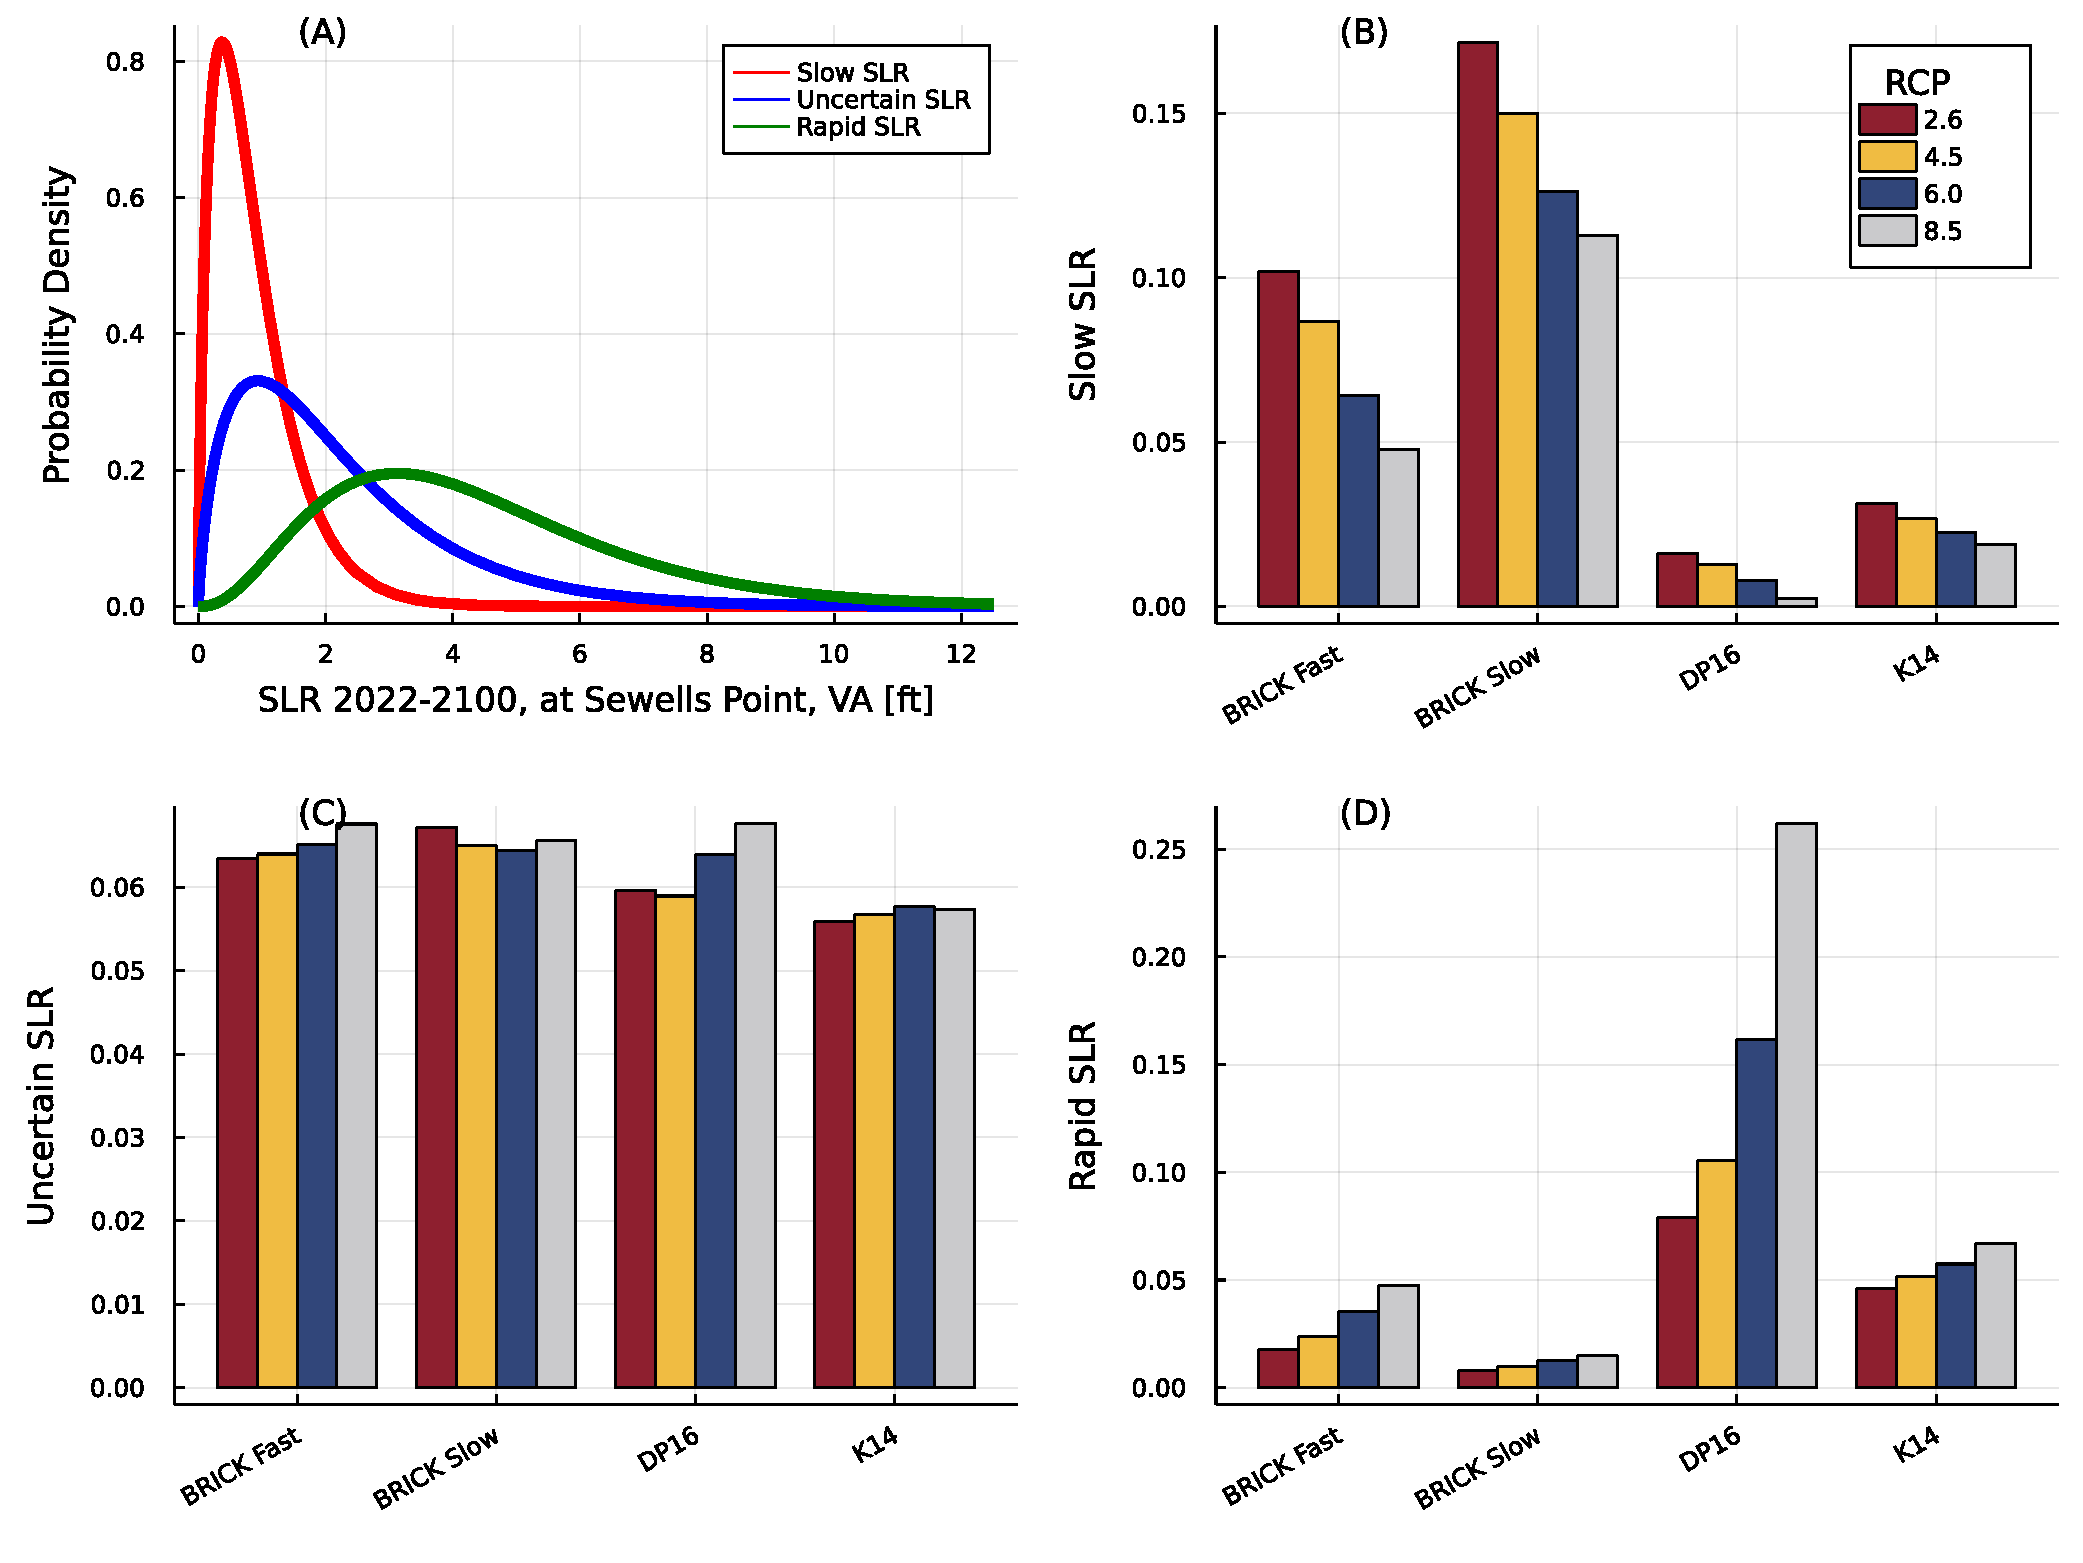
\includegraphics[width=\textwidth]{lsl-priors-weights}
  \caption{
    Impact of subjective priors for local sea level on implicit weight given to each \gls{rcp} scenario and physical model.
    We develop three distributions (``subjective priors'') representing plausible probabilistic beliefs about \gls{msl} at Sewells Point, VA in 2100, relative to the present.
    The \glspl{pdf} of these subjective priors are shown in panel (A).
    In panels (B-C) we show the relationship between these subjective priors and the 16 probabilistic models (four \gls{rcp} scenarios and four physical representations) available.
    Specifically, (B-C) show the average weight given to each model by each of the subjective priors.
  }\label{fig:lsl-priors-weights}
\end{figure}

One application of this method is to diagnose which assumptions different $p_\mathrm{belief}$ are consistent with.
\Cref{fig:lsl-priors-weights}(B-D) shows the total weight that each prior assigns to \glspl{sow} generated by each \gls{rcp} scenario and physical model.
For example, the rapid \gls{slr} scenario (green line in \cref{fig:lsl-priors-weights}) places most weight on the DP16 model, and particularly on \gls{rcp} 8.5 which by some accounts is unlikely given current policy \cite{hausfather_scenarios:2020,srikrishnan_probabilistic:2022}.
Conversely, the slow \gls{slr} scenario (red line) places most weight on the BRICK models, particularly \gls{rcp} 2.6 \cite<also unlikely given current policy;>{hausfather_scenarios:2020,srikrishnan_probabilistic:2022}) and \gls{rcp} 4.5.
The uncertain \gls{slr} scenario (blue line) allocates approximately equal weight across models.

This method can also be used to calculate expectations, allowing us to revisit the trade-off diagrams of \cref{fig:tradeoffs-by-rcp}.
\Cref{fig:tradeoffs-by-prior} shows the total lifetime cost (panel A) and lifetime expected damages (panel B) under each model.
Notably, they give different guidance.
Under an assumption of rapid \gls{slr}, elevating the house by approximately \SI{6}{ft} costs 73\% of house value and reduces damages by over 100\% of house value, yielding a benefit to cost ratio of approximately 1.25.
Under an assumption of slow \gls{slr}, the same decision reduces damages only by 50\% of house value, yielding a benefit to cost ratio of approximately 0.7.
Under the intermediate / uncertain \gls{slr} assumption, the expected lifetime costs are similar for elevating or not elevating the house, and thus the benefit to cost ratio is nearly 1.
Under all assumptions, elevating by only a few feet is impractical because it involves paying the large fixed costs of elevation (\cref{fig:cost-up-front}) but offers relatively little flood reduction.

\begin{figure}
  \centering
  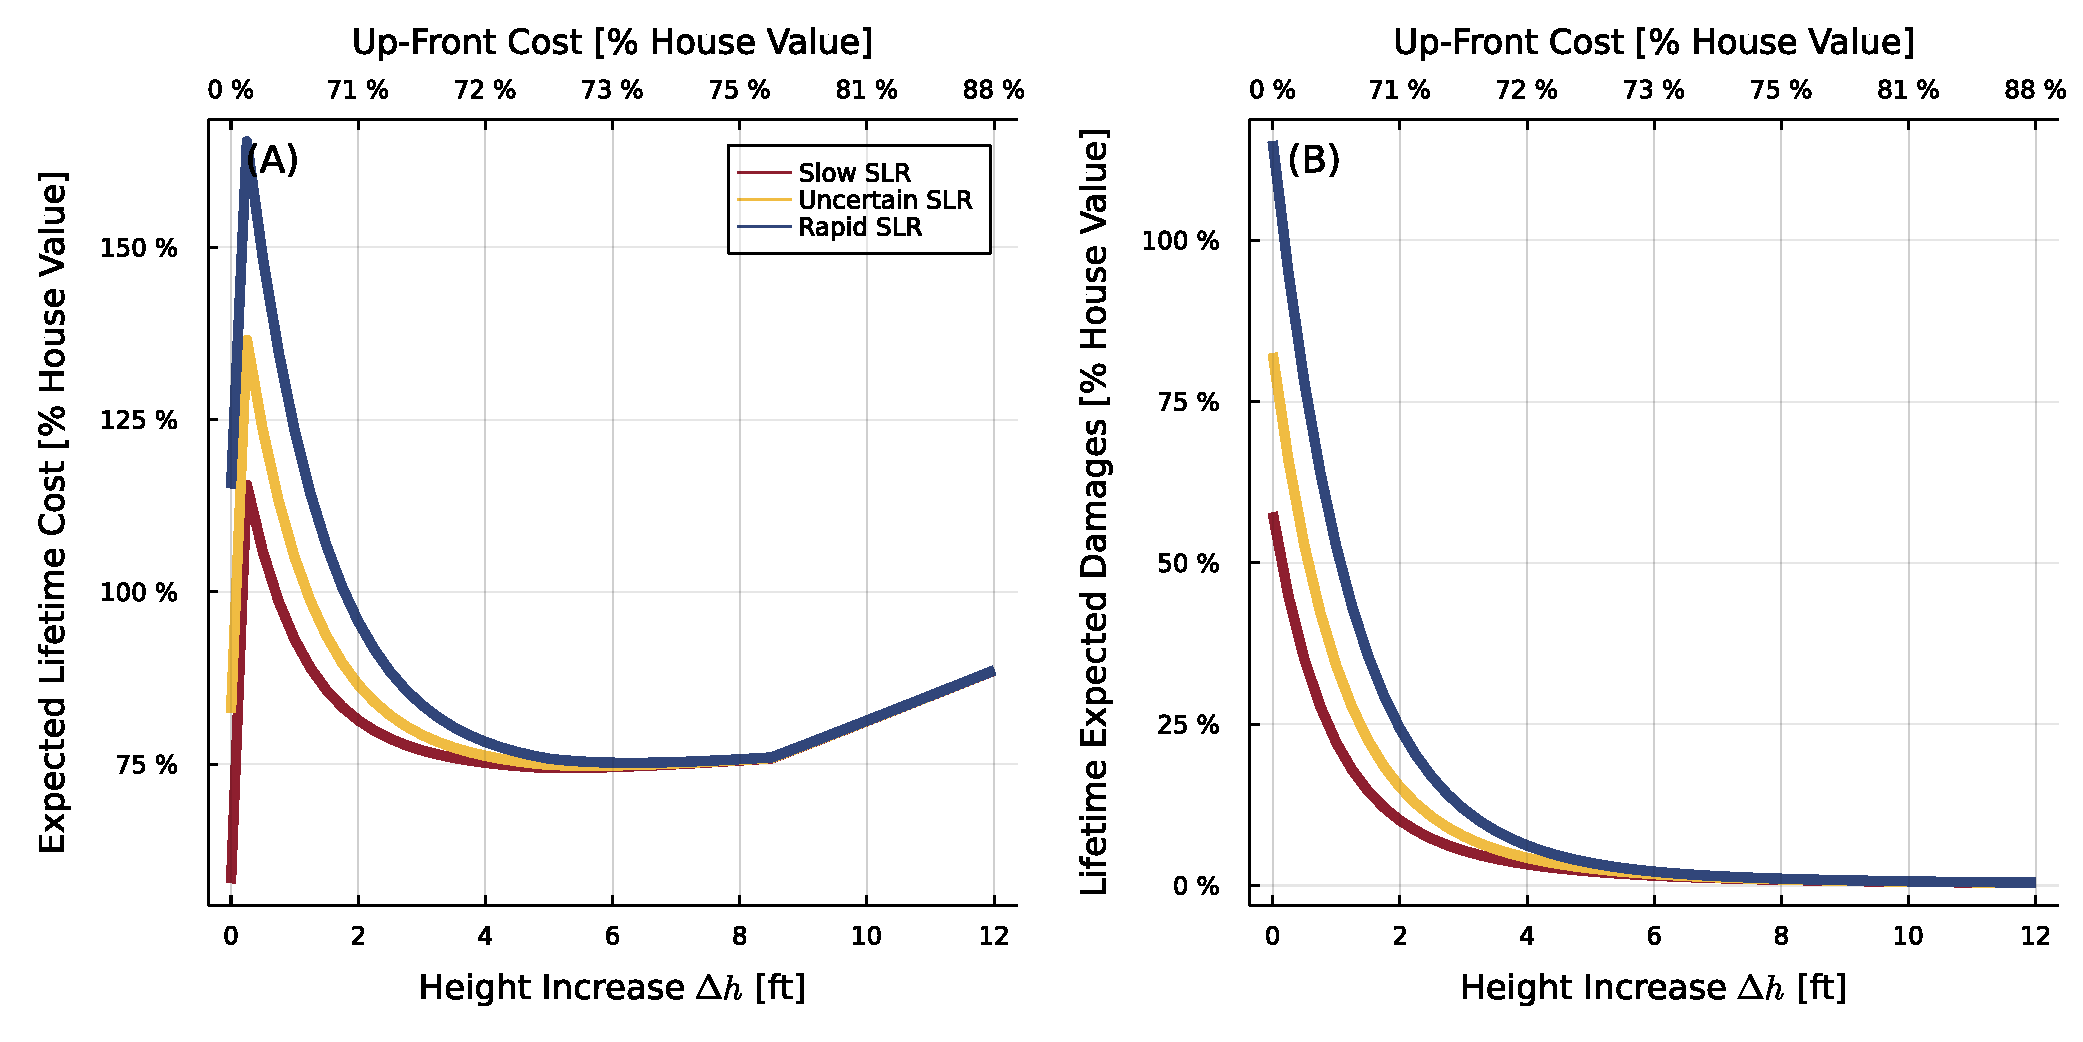
\includegraphics[width=\textwidth]{tradeoffs-by-prior}
  \caption{
    As \cref{fig:tradeoffs-by-rcp}, but with Pareto frontiers for the full distribution of outcomes using the three models of $p_\mathrm{belief}$ (colors).
  }\label{fig:tradeoffs-by-prior}
\end{figure}

\section{Discussion and research needs}\label{sec:caveats}

Several limitations to our study merit further discussion.
The first category has to do with limitations of the underlying method proposed for re-weighting \glspl{sow}.
For example, we develop a subjective prior belief $p_\mathrm{belief}(\Psi)$ over \gls{msl} in the year 2100.
Although this is a low-dimensional representation of the full time series, it is not a sufficient statistic; prior studies have shown that using Approximate Bayesian Computation to calibrate models on low dimensional statistics using that are not sufficient statistics can lead to biased posterior estimates \cite{csillery_abc:2010,marjoram_abc:2006}.
Although we are not performing calibration here, and this is thus not a direct concern, time series with the same \gls{msl} in 2100 may differ in other ways, and experts may have prior information about the likelihood of these differences not represented in our model.
A related concern is that we developed our three distributions for $p_\mathrm{belief}(\Psi)$  in an \emph{ad hoc} fashion that may not represent well-calibrated beliefs.
Although this is appropriate for our didactic illustration, recent advances in Bayesian elicitation of expert opinion \cite<see>[and references therein]{mikkola_elicitation:2021} can be applied to improve decision making in real world case studies.
More fundamentally, our method assumes that there exists an expert capable of integrating over the many processes that drive \gls{slr}, from global greenhouse gas emissions to the global carbon cycle to climate sensitivity and ice sheet response \cite{morgan_elicitation:2014}.
An alternative approach would be to build a probabilistic model for each of these steps, and to use each as an input to the next to develop a fully probabilistic model for \gls{slr}.
Yet while some progress has been made developing probabilistic models for specific elements of this model chain \cite<\eg,>[]{srikrishnan_probabilistic:2022,wong_brick0.2:2017}, this remains a computational and conceptual challenge.
Finally, while our aim in this paper has been to demonstrate the value of integrating Bayesian workflow \cite{gelman_workflow:2020} into \gls{dmdu}, further work is needed to improve this integration.

The second category of limitations has to do with the case study and our interpretation of the house elevation decision problem.
This problem intersects with decisions about where to live and how to manage household finances, both of which are highly complex.
One extension of our analysis would be to consider additional decision objectives.
In particular, we hypothesize that incorporating improved representations of risk aversion into decision support may substantially improve their usability.
One could also extend the analysis to consider additional sources of uncertainty such as depth-damage relationships \cite{Rozer:2019,nofal_fragility:2020}, the cost of elevating a house, the house lifespan, the effective discount rate, and value of the land on which the house is built \cite[provides a framework for addressing some of these]{zarekarizi_suboptimal:2020}.
Finally, while here we consider the decision to be a one-time decision, one could also frame this as problem a sequential decision.
The analysis of sequential decision problems applies tools from control theory and reinforcement learning to identify policies that map ``triggers'' (\ie, state variables) to decisions \cite{herman_control:2020}.
Yet although framing the decision through a sequential lens can increase adaptability and improve outcomes \cite{fletcher:2017,garner_slrise:2018}, the optimized policy rules are necessarily sensitive to the characterization of uncertainty, and thus the problem of synthesizing across deep uncertainties remains \cite{herman_control:2020}.

These limitations motivate several directions for future research.
From a methodological perspective, developing model chains that capture uncertainties in global energy and economic pathways, global climate sensitivity, and local hazard response \cite<see fig.~1 of>[]{moss_uncertainties:2000} offers a principled framework for fully probabilistic estimation of local hazard, subject to (still necessarily subjective) priors over key parameters.
From a decision support perspective, improved understanding of the conditions under which household-scale strategies for flood risk management, like elevation, achieve relevant objectives could support improved resilience and adaptation.
Additionally, since developing bespoke analyses for each house may be impractical, identifying decision rules that are applicable across different house characteristics may improve usability.

\section{Conclusions}\label{sec:conclusions}

This study develops a framework designed to increase the transparency of quantitative decision analysis under deep uncertainty.
We develop a framework capable of blending iterative, stakeholder-driven exploratory modeling with subjective probabilistic expert assessment.
Such an approach is urgently needed given that deeply uncertain nonstationarity hazards pose a fundamental challenge to classical methods of hazard estimation.
We use a didactic case study of house elevation in the coastal zone to illustrate a method for transparently synthesizing across deep uncertainties.

The proposed scenario weighting framework can be applied to inform critical challenges in climate risk management.
An obvious area of application is to the design of infrastructure.
For example, much of the stormwater infrastructure in the United States is inadequate for current and anticipated future climates \cite{lopez-cantu:2018}.
Yet upgrading this infrastructure is costly and subject to large uncertainties between rainfall models \cite{sharma_rcp:2021} and \gls{rcp} scenarios.
Similarly, decisions like  levee heightening \cite{garner_slrise:2018,oddo_coastal:2017,vandantzig_dike:1956} and sea wall design (as discussed in the Introduction) are subject to deep uncertainties in sea level rise.
Investments in water resources planning and management depend on assumptions of future water demand, availability, and technologies \cite{trindade_deeplyuncertainpathways:2019}.
And analyses of climate change mitigation options, such as estimates of the social cost of pollutants \cite{errickson_methane:2021} or cost-minimizing energy transition pathways, are conditional on probabilistic models for inputs like technology prices and population.

Of course, all models are ultimately wrong \cite{box_sciencestatistics:1976}.
Thus seeking decisions that perform well across a range of assumptions, and improving the decision space through robust design and flexibility, can improve outcomes.
Yet whenever decisions are compared quantitatively, assumptions about the probability of different possible futures are necessarily made.
We call for researchers studying climate risk management to make these implicit assumptions explicit, and we suggest that coordinated guidance can help practitioners determine better design criteria.

\section{Open Research}

All code, including source code, is available under the GNU Public License (version 3) at \url{https://github.com/jdossgollin/2022-elevation-robustness}.
This code is written in the open source Julia programming language and detailed instructions for reproducing our results are provided.
A permanent, citeable archive of the precise version of the codes used in this study is also available on Zenodo at \url{https://doi.org/10.5281/zenodo.6814588}.

%%%%%%%%%%%%%%%%%%%%%%%%%%%%%%%%%%%%%%%%%%%%%%%

\acknowledgments

This work was supported by \acrfull{noaa} through the Mid-Atlantic Regional Integrated Sciences and Assessments (MARISA) program under \gls{noaa} grant NA16OAR4310179 and through the Penn State Initiative for Resilient Communities (PSIRC) by a Strategic Plan seed grant from the Penn State Office of the Provost, with co-support from the Center for Climate Risk Management (CLIMA), the Rock Ethics Institute, Penn State Law, and the Hamer Center for Community Design.
JDG thanks Rice University for support.
KK thanks Dartmouth College for support.
The authors thank
Sitara Baboolal,
Tor Erlend Fjelde,
Catalina González-Dueñas,
Adam Pollack,
and
Vivek Srikrishnan
for helpful comments.


%% ------------------------------------------------------------------------ %%
%% References and Citations
% don't specify bibliographystyle
% In the References section, cite the data/software described in the Availability Statement (this includes primary and processed data used for your research). For details on data/software citation as well as examples, see the Data & Software Citation section of the Data & Software for Authors guidance
% https://www.agu.org/Publish-with-AGU/Publish/Author-Resources/Data-and-Software-for-Authors#citation

%%%%%%%%%%%%%%%%%%%%%%%%%%%%%%%%%%%%%%%%%%%%%%%

\bibliography{library-bibtex}


\end{document}
